\documentclass[1p]{elsarticle_modified}
%\bibliographystyle{elsarticle-num}

%\usepackage[colorlinks]{hyperref}
%\usepackage{abbrmath_seonhwa} %\Abb, \Ascr, \Acal ,\Abf, \Afrak
\usepackage{amsfonts}
\usepackage{amssymb}
\usepackage{amsmath}
\usepackage{amsthm}
\usepackage{scalefnt}
\usepackage{amsbsy}
\usepackage{kotex}
\usepackage{caption}
\usepackage{subfig}
\usepackage{color}
\usepackage{graphicx}
\usepackage{xcolor} %% white, black, red, green, blue, cyan, magenta, yellow
\usepackage{float}
\usepackage{setspace}
\usepackage{hyperref}

\usepackage{tikz}
\usetikzlibrary{arrows}

\usepackage{multirow}
\usepackage{array} % fixed length table
\usepackage{hhline}

%%%%%%%%%%%%%%%%%%%%%
\makeatletter
\renewcommand*\env@matrix[1][\arraystretch]{%
	\edef\arraystretch{#1}%
	\hskip -\arraycolsep
	\let\@ifnextchar\new@ifnextchar
	\array{*\c@MaxMatrixCols c}}
\makeatother %https://tex.stackexchange.com/questions/14071/how-can-i-increase-the-line-spacing-in-a-matrix
%%%%%%%%%%%%%%%

\usepackage[normalem]{ulem}

\newcommand{\msout}[1]{\ifmmode\text{\sout{\ensuremath{#1}}}\else\sout{#1}\fi}
%SOURCE: \msout is \stkout macro in https://tex.stackexchange.com/questions/20609/strikeout-in-math-mode

\newcommand{\cancel}[1]{
	\ifmmode
	{\color{red}\msout{#1}}
	\else
	{\color{red}\sout{#1}}
	\fi
}

\newcommand{\add}[1]{
	{\color{blue}\uwave{#1}}
}

\newcommand{\replace}[2]{
	\ifmmode
	{\color{red}\msout{#1}}{\color{blue}\uwave{#2}}
	\else
	{\color{red}\sout{#1}}{\color{blue}\uwave{#2}}
	\fi
}

\newcommand{\Sol}{\mathcal{S}} %segment
\newcommand{\D}{D} %diagram
\newcommand{\A}{\mathcal{A}} %arc


%%%%%%%%%%%%%%%%%%%%%%%%%%%%%5 test

\def\sl{\operatorname{\textup{SL}}(2,\Cbb)}
\def\psl{\operatorname{\textup{PSL}}(2,\Cbb)}
\def\quan{\mkern 1mu \triangleright \mkern 1mu}

\theoremstyle{definition}
\newtheorem{thm}{Theorem}[section]
\newtheorem{prop}[thm]{Proposition}
\newtheorem{lem}[thm]{Lemma}
\newtheorem{ques}[thm]{Question}
\newtheorem{cor}[thm]{Corollary}
\newtheorem{defn}[thm]{Definition}
\newtheorem{exam}[thm]{Example}
\newtheorem{rmk}[thm]{Remark}
\newtheorem{alg}[thm]{Algorithm}

\newcommand{\I}{\sqrt{-1}}
\begin{document}

%\begin{frontmatter}
%
%\title{Boundary parabolic representations of knots up to 8 crossings}
%
%%% Group authors per affiliation:
%\author{Yunhi Cho} 
%\address{Department of Mathematics, University of Seoul, Seoul, Korea}
%\ead{yhcho@uos.ac.kr}
%
%
%\author{Seonhwa Kim} %\fnref{s_kim}}
%\address{Center for Geometry and Physics, Institute for Basic Science, Pohang, 37673, Korea}
%\ead{ryeona17@ibs.re.kr}
%
%\author{Hyuk Kim}
%\address{Department of Mathematical Sciences, Seoul National University, Seoul 08826, Korea}
%\ead{hyukkim@snu.ac.kr}
%
%\author{Seokbeom Yoon}
%\address{Department of Mathematical Sciences, Seoul National University, Seoul, 08826,  Korea}
%\ead{sbyoon15@snu.ac.kr}
%
%\begin{abstract}
%We find all boundary parabolic representation of knots up to 8 crossings.
%
%\end{abstract}
%\begin{keyword}
%    \MSC[2010] 57M25 
%\end{keyword}
%
%\end{frontmatter}

%\linenumbers
%\tableofcontents
%
\newcommand\colored[1]{\textcolor{white}{\rule[-0.35ex]{0.8em}{1.4ex}}\kern-0.8em\color{red} #1}%
%\newcommand\colored[1]{\textcolor{white}{ #1}\kern-2.17ex	\textcolor{white}{ #1}\kern-1.81ex	\textcolor{white}{ #1}\kern-2.15ex\color{red}#1	}

{\Large $\underline{12a_{0807}~(K12a_{0807})}$}

\setlength{\tabcolsep}{10pt}
\renewcommand{\arraystretch}{1.6}
\vspace{1cm}\begin{tabular}{m{100pt}>{\centering\arraybackslash}m{274pt}}
\multirow{5}{120pt}{
	\centering
	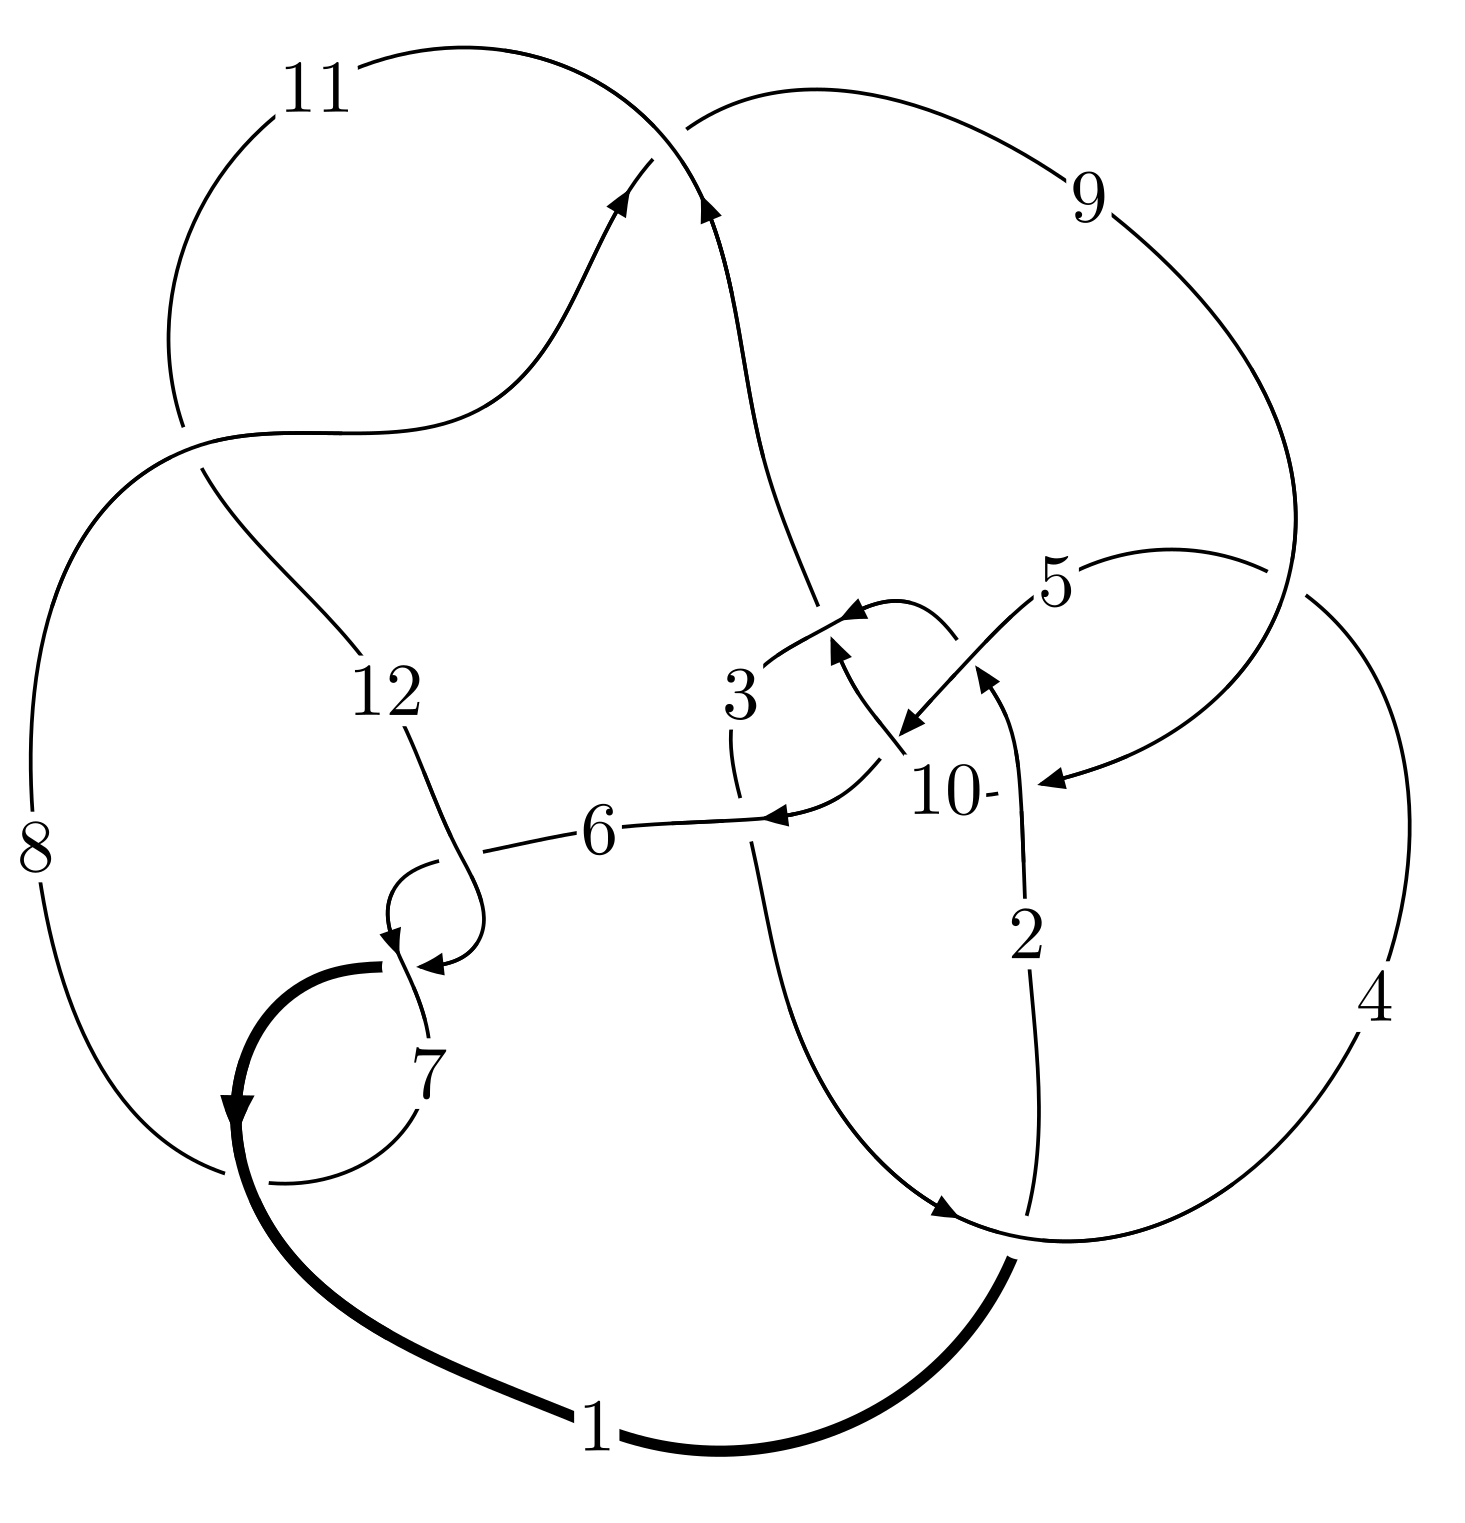
\includegraphics[width=112pt]{../../../GIT/diagram.site/Diagrams/png/1608_12a_0807.png}\\
\ \ \ A knot diagram\footnotemark}&
\allowdisplaybreaks
\textbf{Linearized knot diagam} \\
\cline{2-2}
 &
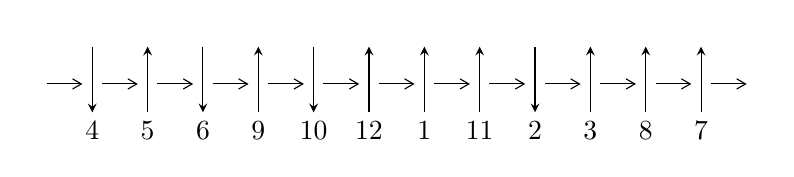
\begin{tikzpicture}[x=20pt, y=17pt]
	% nodes
	\node (C0) at (0, 0) {};
	\node (C1) at (1, 0) {};
	\node (C1U) at (1, +1) {};
	\node (C1D) at (1, -1) {4};

	\node (C2) at (2, 0) {};
	\node (C2U) at (2, +1) {};
	\node (C2D) at (2, -1) {5};

	\node (C3) at (3, 0) {};
	\node (C3U) at (3, +1) {};
	\node (C3D) at (3, -1) {6};

	\node (C4) at (4, 0) {};
	\node (C4U) at (4, +1) {};
	\node (C4D) at (4, -1) {9};

	\node (C5) at (5, 0) {};
	\node (C5U) at (5, +1) {};
	\node (C5D) at (5, -1) {10};

	\node (C6) at (6, 0) {};
	\node (C6U) at (6, +1) {};
	\node (C6D) at (6, -1) {12};

	\node (C7) at (7, 0) {};
	\node (C7U) at (7, +1) {};
	\node (C7D) at (7, -1) {1};

	\node (C8) at (8, 0) {};
	\node (C8U) at (8, +1) {};
	\node (C8D) at (8, -1) {11};

	\node (C9) at (9, 0) {};
	\node (C9U) at (9, +1) {};
	\node (C9D) at (9, -1) {2};

	\node (C10) at (10, 0) {};
	\node (C10U) at (10, +1) {};
	\node (C10D) at (10, -1) {3};

	\node (C11) at (11, 0) {};
	\node (C11U) at (11, +1) {};
	\node (C11D) at (11, -1) {8};

	\node (C12) at (12, 0) {};
	\node (C12U) at (12, +1) {};
	\node (C12D) at (12, -1) {7};
	\node (C13) at (13, 0) {};

	% arrows
	\draw[->,>={angle 60}]
	(C0) edge (C1) (C1) edge (C2) (C2) edge (C3) (C3) edge (C4) (C4) edge (C5) (C5) edge (C6) (C6) edge (C7) (C7) edge (C8) (C8) edge (C9) (C9) edge (C10) (C10) edge (C11) (C11) edge (C12) (C12) edge (C13) ;	\draw[->,>=stealth]
	(C1U) edge (C1D) (C2D) edge (C2U) (C3U) edge (C3D) (C4D) edge (C4U) (C5U) edge (C5D) (C6D) edge (C6U) (C7D) edge (C7U) (C8D) edge (C8U) (C9U) edge (C9D) (C10D) edge (C10U) (C11D) edge (C11U) (C12D) edge (C12U) ;
	\end{tikzpicture} \\
\hhline{~~} \\& 
\textbf{Solving Sequence} \\ \cline{2-2} 
 &
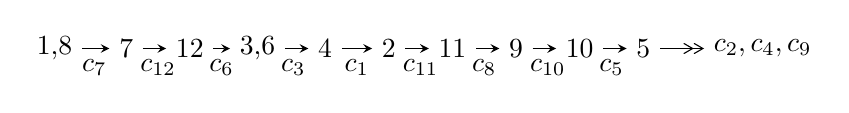
\begin{tikzpicture}[x=23pt, y=7pt]
	% node
	\node (A0) at (-1/8, 0) {1,8};
	\node (A1) at (1, 0) {7};
	\node (A2) at (2, 0) {12};
	\node (A3) at (49/16, 0) {3,6};
	\node (A4) at (33/8, 0) {4};
	\node (A5) at (41/8, 0) {2};
	\node (A6) at (49/8, 0) {11};
	\node (A7) at (57/8, 0) {9};
	\node (A8) at (65/8, 0) {10};
	\node (A9) at (73/8, 0) {5};
	\node (C1) at (1/2, -1) {$c_{7}$};
	\node (C2) at (3/2, -1) {$c_{12}$};
	\node (C3) at (5/2, -1) {$c_{6}$};
	\node (C4) at (29/8, -1) {$c_{3}$};
	\node (C5) at (37/8, -1) {$c_{1}$};
	\node (C6) at (45/8, -1) {$c_{11}$};
	\node (C7) at (53/8, -1) {$c_{8}$};
	\node (C8) at (61/8, -1) {$c_{10}$};
	\node (C9) at (69/8, -1) {$c_{5}$};
	\node (A10) at (11, 0) {$c_{2},c_{4},c_{9}$};

	% edge
	\draw[->,>=stealth]	
	(A0) edge (A1) (A1) edge (A2) (A2) edge (A3) (A3) edge (A4) (A4) edge (A5) (A5) edge (A6) (A6) edge (A7) (A7) edge (A8) (A8) edge (A9) ;
	\draw[->>,>={angle 60}]	
	(A9) edge (A10);
\end{tikzpicture} \\ 

\end{tabular} \\

\footnotetext{
The image of knot diagram is generated by the software ``\textbf{Draw programme}" developed by Andrew Bartholomew(\url{http://www.layer8.co.uk/maths/draw/index.htm\#Running-draw}), where we modified some parts for our purpose(\url{https://github.com/CATsTAILs/LinksPainter}).
}\phantom \\ \newline 
\centering \textbf{Ideals for irreducible components\footnotemark of $X_{\text{par}}$} 
 
\begin{align*}
I^u_{1}&=\langle 
49791514 u^{59}+185733104 u^{58}+\cdots+664747 b+436245750,\\
\phantom{I^u_{1}}&\phantom{= \langle  }5475421 u^{59}+31624832 u^{58}+\cdots+7312217 a+58998547,\;u^{60}+5 u^{59}+\cdots-38 u+11\rangle \\
I^u_{2}&=\langle 
-2861 u^{38} a-1053 u^{38}+\cdots-2113 a-517,\;- u^{38} a+u^{38}+\cdots-3 a-5,\;u^{39}-2 u^{38}+\cdots+2 u-1\rangle \\
I^u_{3}&=\langle 
3 u^{21}-2 u^{20}+\cdots+b-2,\;- u^{21}+u^{20}+\cdots+a+4,\;u^{22}-2 u^{21}+\cdots+u+1\rangle \\
I^u_{4}&=\langle 
b^2+b-1,\;a-1,\;u+1\rangle \\
\\
I^v_{1}&=\langle 
a,\;b+1,\;v-1\rangle \\
\end{align*}
\raggedright * 5 irreducible components of $\dim_{\mathbb{C}}=0$, with total 163 representations.\\
\footnotetext{All coefficients of polynomials are rational numbers. But the coefficients are sometimes approximated in decimal forms when there is not enough margin.}
\newpage
\renewcommand{\arraystretch}{1}
\centering \section*{I. $I^u_{1}= \langle 4.98\times10^{7} u^{59}+1.86\times10^{8} u^{58}+\cdots+6.65\times10^{5} b+4.36\times10^{8},\;5.48\times10^{6} u^{59}+3.16\times10^{7} u^{58}+\cdots+7.31\times10^{6} a+5.90\times10^{7},\;u^{60}+5 u^{59}+\cdots-38 u+11 \rangle$}
\flushleft \textbf{(i) Arc colorings}\\
\begin{tabular}{m{7pt} m{180pt} m{7pt} m{180pt} }
\flushright $a_{1}=$&$\begin{pmatrix}0\\u\end{pmatrix}$ \\
\flushright $a_{8}=$&$\begin{pmatrix}1\\0\end{pmatrix}$ \\
\flushright $a_{7}=$&$\begin{pmatrix}1\\u^2\end{pmatrix}$ \\
\flushright $a_{12}=$&$\begin{pmatrix}- u\\- u^3+u\end{pmatrix}$ \\
\flushright $a_{3}=$&$\begin{pmatrix}-0.748805 u^{59}-4.32493 u^{58}+\cdots+52.3418 u-8.06849\\-74.9030 u^{59}-279.404 u^{58}+\cdots+2793.44 u-656.258\end{pmatrix}$ \\
\flushright $a_{6}=$&$\begin{pmatrix}- u^2+1\\- u^4+2 u^2\end{pmatrix}$ \\
\flushright $a_{4}=$&$\begin{pmatrix}42.7214 u^{59}+157.014 u^{58}+\cdots-1466.48 u+353.804\\-102.962 u^{59}-379.700 u^{58}+\cdots+3682.85 u-871.934\end{pmatrix}$ \\
\flushright $a_{2}=$&$\begin{pmatrix}-34.9557 u^{59}-124.857 u^{58}+\cdots+1080.98 u-269.488\\46.2308 u^{59}+165.630 u^{58}+\cdots-1559.60 u+373.881\end{pmatrix}$ \\
\flushright $a_{11}=$&$\begin{pmatrix}u^3-2 u\\- u^3+u\end{pmatrix}$ \\
\flushright $a_{9}=$&$\begin{pmatrix}u^6-3 u^4+2 u^2+1\\- u^6+2 u^4- u^2\end{pmatrix}$ \\
\flushright $a_{10}=$&$\begin{pmatrix}4.60523 u^{59}+17.8774 u^{58}+\cdots-165.454 u+35.6621\\-42.1101 u^{59}-161.731 u^{58}+\cdots+1740.73 u-400.478\end{pmatrix}$ \\
\flushright $a_{5}=$&$\begin{pmatrix}7.80133 u^{59}+27.2592 u^{58}+\cdots-208.204 u+54.6615\\-73.4028 u^{59}-275.257 u^{58}+\cdots+2770.22 u-651.201\end{pmatrix}$\\&\end{tabular}
\flushleft \textbf{(ii) Obstruction class $= -1$}\\~\\
\flushleft \textbf{(iii) Cusp Shapes $= -\frac{121118688}{664747} u^{59}-\frac{439577769}{664747} u^{58}+\cdots+\frac{4220306946}{664747} u-\frac{1004828410}{664747}$}\\~\\
\newpage\renewcommand{\arraystretch}{1}
\flushleft \textbf{(iv) u-Polynomials at the component}\newline \\
\begin{tabular}{m{50pt}|m{274pt}}
Crossings & \hspace{64pt}u-Polynomials at each crossing \\
\hline $$\begin{aligned}c_{1},c_{3}\end{aligned}$$&$\begin{aligned}
&u^{60}+8 u^{59}+\cdots-27 u+1
\end{aligned}$\\
\hline $$\begin{aligned}c_{2}\end{aligned}$$&$\begin{aligned}
&u^{60}+34 u^{59}+\cdots-87 u-11
\end{aligned}$\\
\hline $$\begin{aligned}c_{4},c_{10}\end{aligned}$$&$\begin{aligned}
&u^{60}+17 u^{56}+\cdots+7 u+1
\end{aligned}$\\
\hline $$\begin{aligned}c_{5},c_{9}\end{aligned}$$&$\begin{aligned}
&u^{60}- u^{59}+\cdots+4 u-1
\end{aligned}$\\
\hline $$\begin{aligned}c_{6},c_{7},c_{12}\end{aligned}$$&$\begin{aligned}
&u^{60}-5 u^{59}+\cdots+38 u+11
\end{aligned}$\\
\hline $$\begin{aligned}c_{8},c_{11}\end{aligned}$$&$\begin{aligned}
&u^{60}+15 u^{59}+\cdots-25484 u-1639
\end{aligned}$\\
\hline
\end{tabular}\\~\\
\newpage\renewcommand{\arraystretch}{1}
\flushleft \textbf{(v) Riley Polynomials at the component}\newline \\
\begin{tabular}{m{50pt}|m{274pt}}
Crossings & \hspace{64pt}Riley Polynomials at each crossing \\
\hline $$\begin{aligned}c_{1},c_{3}\end{aligned}$$&$\begin{aligned}
&y^{60}-44 y^{59}+\cdots-175 y+1
\end{aligned}$\\
\hline $$\begin{aligned}c_{2}\end{aligned}$$&$\begin{aligned}
&y^{60}+58 y^{58}+\cdots-1409 y+121
\end{aligned}$\\
\hline $$\begin{aligned}c_{4},c_{10}\end{aligned}$$&$\begin{aligned}
&y^{60}+34 y^{58}+\cdots-55 y+1
\end{aligned}$\\
\hline $$\begin{aligned}c_{5},c_{9}\end{aligned}$$&$\begin{aligned}
&y^{60}-25 y^{59}+\cdots-66 y+1
\end{aligned}$\\
\hline $$\begin{aligned}c_{6},c_{7},c_{12}\end{aligned}$$&$\begin{aligned}
&y^{60}-51 y^{59}+\cdots-674 y+121
\end{aligned}$\\
\hline $$\begin{aligned}c_{8},c_{11}\end{aligned}$$&$\begin{aligned}
&y^{60}+41 y^{59}+\cdots-39182108 y+2686321
\end{aligned}$\\
\hline
\end{tabular}\\~\\
\newpage\flushleft \textbf{(vi) Complex Volumes and Cusp Shapes}
$$\begin{array}{c|c|c}  
\text{Solutions to }I^u_{1}& \I (\text{vol} + \sqrt{-1}CS) & \text{Cusp shape}\\
 \hline 
\begin{aligned}
u &= \phantom{-}0.060897 + 0.868711 I \\
a &= \phantom{-}1.74244 + 0.72857 I \\
b &= -1.61713 - 0.67161 I\end{aligned}
 & -8.13893 - 2.83634 I & -3.79343 + 3.27629 I \\ \hline\begin{aligned}
u &= \phantom{-}0.060897 - 0.868711 I \\
a &= \phantom{-}1.74244 - 0.72857 I \\
b &= -1.61713 + 0.67161 I\end{aligned}
 & -8.13893 + 2.83634 I & -3.79343 - 3.27629 I \\ \hline\begin{aligned}
u &= \phantom{-}0.128834 + 0.848151 I \\
a &= \phantom{-}3.09604 - 0.05310 I \\
b &= -2.55532 + 0.53851 I\end{aligned}
 & -5.9522 + 14.9479 I & \phantom{-0.000000 } 0. - 8.67429 I \\ \hline\begin{aligned}
u &= \phantom{-}0.128834 - 0.848151 I \\
a &= \phantom{-}3.09604 + 0.05310 I \\
b &= -2.55532 - 0.53851 I\end{aligned}
 & -5.9522 - 14.9479 I & \phantom{-0.000000 -}0. + 8.67429 I \\ \hline\begin{aligned}
u &= \phantom{-}0.095160 + 0.812795 I \\
a &= -3.40389 + 0.06404 I \\
b &= \phantom{-}2.60895 - 0.21567 I\end{aligned}
 & -6.77759 + 6.06790 I & -6.89903 - 8.29238 I \\ \hline\begin{aligned}
u &= \phantom{-}0.095160 - 0.812795 I \\
a &= -3.40389 - 0.06404 I \\
b &= \phantom{-}2.60895 + 0.21567 I\end{aligned}
 & -6.77759 - 6.06790 I & -6.89903 + 8.29238 I \\ \hline\begin{aligned}
u &= \phantom{-}1.139700 + 0.336402 I \\
a &= \phantom{-}1.40739 + 0.67616 I \\
b &= -1.16674 + 1.01101 I\end{aligned}
 & -3.09648 + 1.54338 I & \phantom{-0.000000 } 0 \\ \hline\begin{aligned}
u &= \phantom{-}1.139700 - 0.336402 I \\
a &= \phantom{-}1.40739 - 0.67616 I \\
b &= -1.16674 - 1.01101 I\end{aligned}
 & -3.09648 - 1.54338 I & \phantom{-0.000000 } 0 \\ \hline\begin{aligned}
u &= \phantom{-}0.121157 + 0.797619 I \\
a &= -2.01479 - 1.24838 I \\
b &= \phantom{-}1.55370 + 0.68878 I\end{aligned}
 & -6.18372 + 2.58960 I & -4.84200 - 1.19126 I \\ \hline\begin{aligned}
u &= \phantom{-}0.121157 - 0.797619 I \\
a &= -2.01479 + 1.24838 I \\
b &= \phantom{-}1.55370 - 0.68878 I\end{aligned}
 & -6.18372 - 2.58960 I & -4.84200 + 1.19126 I\\
 \hline 
 \end{array}$$\newpage$$\begin{array}{c|c|c}  
\text{Solutions to }I^u_{1}& \I (\text{vol} + \sqrt{-1}CS) & \text{Cusp shape}\\
 \hline 
\begin{aligned}
u &= \phantom{-}1.123550 + 0.412628 I \\
a &= -0.72460 - 1.64385 I \\
b &= \phantom{-}2.25070 + 0.01928 I\end{aligned}
 & -2.90687 - 10.41390 I & \phantom{-0.000000 } 0 \\ \hline\begin{aligned}
u &= \phantom{-}1.123550 - 0.412628 I \\
a &= -0.72460 + 1.64385 I \\
b &= \phantom{-}2.25070 - 0.01928 I\end{aligned}
 & -2.90687 + 10.41390 I & \phantom{-0.000000 } 0 \\ \hline\begin{aligned}
u &= -1.205960 + 0.012637 I \\
a &= -0.103629 - 0.111372 I \\
b &= \phantom{-}0.787825 + 0.838109 I\end{aligned}
 & \phantom{-}2.13388 - 0.44264 I & \phantom{-0.000000 } 0 \\ \hline\begin{aligned}
u &= -1.205960 - 0.012637 I \\
a &= -0.103629 + 0.111372 I \\
b &= \phantom{-}0.787825 - 0.838109 I\end{aligned}
 & \phantom{-}2.13388 + 0.44264 I & \phantom{-0.000000 } 0 \\ \hline\begin{aligned}
u &= -0.011128 + 0.786562 I \\
a &= -2.68629 - 0.56383 I \\
b &= \phantom{-}1.94930 + 0.99862 I\end{aligned}
 & -5.66611 - 0.17773 I & -4.38219 - 0.43593 I \\ \hline\begin{aligned}
u &= -0.011128 - 0.786562 I \\
a &= -2.68629 + 0.56383 I \\
b &= \phantom{-}1.94930 - 0.99862 I\end{aligned}
 & -5.66611 + 0.17773 I & -4.38219 + 0.43593 I \\ \hline\begin{aligned}
u &= \phantom{-}1.166760 + 0.357089 I \\
a &= \phantom{-}0.97029 + 1.86168 I \\
b &= -2.17056 + 0.36127 I\end{aligned}
 & -3.50603 - 1.83244 I & \phantom{-0.000000 } 0 \\ \hline\begin{aligned}
u &= \phantom{-}1.166760 - 0.357089 I \\
a &= \phantom{-}0.97029 - 1.86168 I \\
b &= -2.17056 - 0.36127 I\end{aligned}
 & -3.50603 + 1.83244 I & \phantom{-0.000000 } 0 \\ \hline\begin{aligned}
u &= \phantom{-}0.548543 + 0.502233 I \\
a &= \phantom{-}0.206746 + 0.433608 I \\
b &= \phantom{-}0.745089 + 0.097408 I\end{aligned}
 & -0.86790 + 10.42950 I & \phantom{-}3.00610 - 9.66598 I \\ \hline\begin{aligned}
u &= \phantom{-}0.548543 - 0.502233 I \\
a &= \phantom{-}0.206746 - 0.433608 I \\
b &= \phantom{-}0.745089 - 0.097408 I\end{aligned}
 & -0.86790 - 10.42950 I & \phantom{-}3.00610 + 9.66598 I\\
 \hline 
 \end{array}$$\newpage$$\begin{array}{c|c|c}  
\text{Solutions to }I^u_{1}& \I (\text{vol} + \sqrt{-1}CS) & \text{Cusp shape}\\
 \hline 
\begin{aligned}
u &= \phantom{-}0.431078 + 0.588336 I \\
a &= \phantom{-}0.023424 + 0.774923 I \\
b &= -0.107206 + 0.378275 I\end{aligned}
 & -1.26191 - 6.52666 I & \phantom{-}1.65444 + 4.13374 I \\ \hline\begin{aligned}
u &= \phantom{-}0.431078 - 0.588336 I \\
a &= \phantom{-}0.023424 - 0.774923 I \\
b &= -0.107206 - 0.378275 I\end{aligned}
 & -1.26191 + 6.52666 I & \phantom{-}1.65444 - 4.13374 I \\ \hline\begin{aligned}
u &= -1.250750 + 0.253692 I \\
a &= -0.602712 + 0.147425 I \\
b &= \phantom{-}1.166760 + 0.424599 I\end{aligned}
 & \phantom{-}1.80106 - 1.18068 I & \phantom{-0.000000 } 0 \\ \hline\begin{aligned}
u &= -1.250750 - 0.253692 I \\
a &= -0.602712 - 0.147425 I \\
b &= \phantom{-}1.166760 - 0.424599 I\end{aligned}
 & \phantom{-}1.80106 + 1.18068 I & \phantom{-0.000000 } 0 \\ \hline\begin{aligned}
u &= -0.077320 + 0.719425 I \\
a &= \phantom{-}1.32124 - 0.56354 I \\
b &= -1.066300 - 0.127595 I\end{aligned}
 & -1.73557 - 2.28005 I & \phantom{-}2.10056 + 2.97528 I \\ \hline\begin{aligned}
u &= -0.077320 - 0.719425 I \\
a &= \phantom{-}1.32124 + 0.56354 I \\
b &= -1.066300 + 0.127595 I\end{aligned}
 & -1.73557 + 2.28005 I & \phantom{-}2.10056 - 2.97528 I \\ \hline\begin{aligned}
u &= \phantom{-}1.206360 + 0.420533 I \\
a &= -1.030210 - 0.819652 I \\
b &= \phantom{-}1.26332 - 1.06914 I\end{aligned}
 & -4.61140 + 7.45006 I & \phantom{-0.000000 } 0 \\ \hline\begin{aligned}
u &= \phantom{-}1.206360 - 0.420533 I \\
a &= -1.030210 + 0.819652 I \\
b &= \phantom{-}1.26332 + 1.06914 I\end{aligned}
 & -4.61140 - 7.45006 I & \phantom{-0.000000 } 0 \\ \hline\begin{aligned}
u &= \phantom{-}1.27903\phantom{ +0.000000I} \\
a &= \phantom{-}1.93254\phantom{ +0.000000I} \\
b &= \phantom{-}0.333489\phantom{ +0.000000I}\end{aligned}
 & \phantom{-}2.37328\phantom{ +0.000000I} & \phantom{-0.000000 } 0 \\ \hline\begin{aligned}
u &= -1.261350 + 0.340608 I \\
a &= \phantom{-}0.411479 - 1.290950 I \\
b &= -2.32788 + 0.56589 I\end{aligned}
 & -1.79214 - 3.88409 I & \phantom{-0.000000 } 0\\
 \hline 
 \end{array}$$\newpage$$\begin{array}{c|c|c}  
\text{Solutions to }I^u_{1}& \I (\text{vol} + \sqrt{-1}CS) & \text{Cusp shape}\\
 \hline 
\begin{aligned}
u &= -1.261350 - 0.340608 I \\
a &= \phantom{-}0.411479 + 1.290950 I \\
b &= -2.32788 - 0.56589 I\end{aligned}
 & -1.79214 + 3.88409 I & \phantom{-0.000000 } 0 \\ \hline\begin{aligned}
u &= -0.385617 + 0.575805 I \\
a &= \phantom{-}0.355886 + 0.193509 I \\
b &= \phantom{-}0.088406 - 0.407822 I\end{aligned}
 & \phantom{-}0.93949 - 1.79577 I & \phantom{-}8.38505 - 1.97163 I \\ \hline\begin{aligned}
u &= -0.385617 - 0.575805 I \\
a &= \phantom{-}0.355886 - 0.193509 I \\
b &= \phantom{-}0.088406 + 0.407822 I\end{aligned}
 & \phantom{-}0.93949 + 1.79577 I & \phantom{-}8.38505 + 1.97163 I \\ \hline\begin{aligned}
u &= \phantom{-}1.278460 + 0.340753 I \\
a &= \phantom{-}1.26291 + 1.54365 I \\
b &= -1.52939 + 1.35909 I\end{aligned}
 & -1.65511 + 4.23939 I & \phantom{-0.000000 } 0 \\ \hline\begin{aligned}
u &= \phantom{-}1.278460 - 0.340753 I \\
a &= \phantom{-}1.26291 - 1.54365 I \\
b &= -1.52939 - 1.35909 I\end{aligned}
 & -1.65511 - 4.23939 I & \phantom{-0.000000 } 0 \\ \hline\begin{aligned}
u &= -1.350340 + 0.079844 I \\
a &= \phantom{-}0.354882 - 0.159748 I \\
b &= \phantom{-}0.55689 + 1.39046 I\end{aligned}
 & \phantom{-}3.39876 - 4.42651 I & \phantom{-0.000000 } 0 \\ \hline\begin{aligned}
u &= -1.350340 - 0.079844 I \\
a &= \phantom{-}0.354882 + 0.159748 I \\
b &= \phantom{-}0.55689 - 1.39046 I\end{aligned}
 & \phantom{-}3.39876 + 4.42651 I & \phantom{-0.000000 } 0 \\ \hline\begin{aligned}
u &= \phantom{-}1.317550 + 0.310044 I \\
a &= -0.263784 - 1.093550 I \\
b &= \phantom{-}0.991089 - 0.453216 I\end{aligned}
 & \phantom{-}2.64360 + 6.02566 I & \phantom{-0.000000 } 0 \\ \hline\begin{aligned}
u &= \phantom{-}1.317550 - 0.310044 I \\
a &= -0.263784 + 1.093550 I \\
b &= \phantom{-}0.991089 + 0.453216 I\end{aligned}
 & \phantom{-}2.64360 - 6.02566 I & \phantom{-0.000000 } 0 \\ \hline\begin{aligned}
u &= \phantom{-}1.35461\phantom{ +0.000000I} \\
a &= -0.906395\phantom{ +0.000000I} \\
b &= -0.361301\phantom{ +0.000000I}\end{aligned}
 & \phantom{-}6.51449\phantom{ +0.000000I} & \phantom{-0.000000 } 0\\
 \hline 
 \end{array}$$\newpage$$\begin{array}{c|c|c}  
\text{Solutions to }I^u_{1}& \I (\text{vol} + \sqrt{-1}CS) & \text{Cusp shape}\\
 \hline 
\begin{aligned}
u &= -1.311420 + 0.396696 I \\
a &= -0.189189 + 1.092900 I \\
b &= \phantom{-}1.76017 - 0.21463 I\end{aligned}
 & -3.85452 - 1.69969 I & \phantom{-0.000000 } 0 \\ \hline\begin{aligned}
u &= -1.311420 - 0.396696 I \\
a &= -0.189189 - 1.092900 I \\
b &= \phantom{-}1.76017 + 0.21463 I\end{aligned}
 & -3.85452 + 1.69969 I & \phantom{-0.000000 } 0 \\ \hline\begin{aligned}
u &= -1.330390 + 0.355574 I \\
a &= \phantom{-}1.26040 - 1.73128 I \\
b &= -2.83443 - 0.72331 I\end{aligned}
 & -2.30463 - 10.27760 I & \phantom{-0.000000 } 0 \\ \hline\begin{aligned}
u &= -1.330390 - 0.355574 I \\
a &= \phantom{-}1.26040 + 1.73128 I \\
b &= -2.83443 + 0.72331 I\end{aligned}
 & -2.30463 + 10.27760 I & \phantom{-0.000000 } 0 \\ \hline\begin{aligned}
u &= -1.38309\phantom{ +0.000000I} \\
a &= \phantom{-}0.187317\phantom{ +0.000000I} \\
b &= \phantom{-}1.04622\phantom{ +0.000000I}\end{aligned}
 & \phantom{-}3.23568\phantom{ +0.000000I} & \phantom{-0.000000 } 0 \\ \hline\begin{aligned}
u &= -1.346470 + 0.343806 I \\
a &= \phantom{-}0.20565 - 1.42562 I \\
b &= -1.73002 + 0.40643 I\end{aligned}
 & -1.56255 - 6.70988 I & \phantom{-0.000000 } 0 \\ \hline\begin{aligned}
u &= -1.346470 - 0.343806 I \\
a &= \phantom{-}0.20565 + 1.42562 I \\
b &= -1.73002 - 0.40643 I\end{aligned}
 & -1.56255 + 6.70988 I & \phantom{-0.000000 } 0 \\ \hline\begin{aligned}
u &= -1.354300 + 0.371721 I \\
a &= -1.20650 + 1.73448 I \\
b &= \phantom{-}2.62599 + 0.98286 I\end{aligned}
 & -1.2861 - 19.3357 I & \phantom{-0.000000 } 0 \\ \hline\begin{aligned}
u &= -1.354300 - 0.371721 I \\
a &= -1.20650 - 1.73448 I \\
b &= \phantom{-}2.62599 - 0.98286 I\end{aligned}
 & -1.2861 + 19.3357 I & \phantom{-0.000000 } 0 \\ \hline\begin{aligned}
u &= -1.41652 + 0.11414 I \\
a &= -0.669108 + 0.142685 I \\
b &= -0.682724 - 0.737781 I\end{aligned}
 & \phantom{-}5.40592 - 12.35690 I & \phantom{-0.000000 } 0\\
 \hline 
 \end{array}$$\newpage$$\begin{array}{c|c|c}  
\text{Solutions to }I^u_{1}& \I (\text{vol} + \sqrt{-1}CS) & \text{Cusp shape}\\
 \hline 
\begin{aligned}
u &= -1.41652 - 0.11414 I \\
a &= -0.669108 - 0.142685 I \\
b &= -0.682724 + 0.737781 I\end{aligned}
 & \phantom{-}5.40592 + 12.35690 I & \phantom{-0.000000 } 0 \\ \hline\begin{aligned}
u &= -1.41428 + 0.17772 I \\
a &= \phantom{-}0.134372 + 0.588151 I \\
b &= -0.272154 + 0.118060 I\end{aligned}
 & \phantom{-}4.63496 + 3.89220 I & \phantom{-0.000000 } 0 \\ \hline\begin{aligned}
u &= -1.41428 - 0.17772 I \\
a &= \phantom{-}0.134372 - 0.588151 I \\
b &= -0.272154 - 0.118060 I\end{aligned}
 & \phantom{-}4.63496 - 3.89220 I & \phantom{-0.000000 } 0 \\ \hline\begin{aligned}
u &= \phantom{-}1.44039 + 0.21474 I \\
a &= -0.309129 - 0.085453 I \\
b &= -0.134108 - 0.270569 I\end{aligned}
 & \phantom{-}6.80384 + 4.70309 I & \phantom{-0.000000 } 0 \\ \hline\begin{aligned}
u &= \phantom{-}1.44039 - 0.21474 I \\
a &= -0.309129 + 0.085453 I \\
b &= -0.134108 + 0.270569 I\end{aligned}
 & \phantom{-}6.80384 - 4.70309 I & \phantom{-0.000000 } 0 \\ \hline\begin{aligned}
u &= \phantom{-}0.403727 + 0.360380 I \\
a &= -0.263367 - 1.336380 I \\
b &= -0.475150 + 0.280630 I\end{aligned}
 & -2.00858 + 3.05776 I & -2.14055 - 8.96943 I \\ \hline\begin{aligned}
u &= \phantom{-}0.403727 - 0.360380 I \\
a &= -0.263367 + 1.336380 I \\
b &= -0.475150 - 0.280630 I\end{aligned}
 & -2.00858 - 3.05776 I & -2.14055 + 8.96943 I \\ \hline\begin{aligned}
u &= \phantom{-}0.359656 + 0.302824 I \\
a &= \phantom{-}1.024700 - 0.936645 I \\
b &= -0.472574 - 0.106407 I\end{aligned}
 & -2.06170 - 0.42298 I & -2.32972 - 0.96462 I \\ \hline\begin{aligned}
u &= \phantom{-}0.359656 - 0.302824 I \\
a &= \phantom{-}1.024700 + 0.936645 I \\
b &= -0.472574 + 0.106407 I\end{aligned}
 & -2.06170 + 0.42298 I & -2.32972 + 0.96462 I \\ \hline\begin{aligned}
u &= -0.462483\phantom{ +0.000000I} \\
a &= \phantom{-}0.619787\phantom{ +0.000000I} \\
b &= \phantom{-}0.568615\phantom{ +0.000000I}\end{aligned}
 & \phantom{-}1.01644\phantom{ +0.000000I} & \phantom{-}10.3330\phantom{ +0.000000I}\\
 \hline 
 \end{array}$$\newpage\newpage\renewcommand{\arraystretch}{1}
\centering \section*{II. $I^u_{2}= \langle -2861 u^{38} a-1053 u^{38}+\cdots-2113 a-517,\;- u^{38} a+u^{38}+\cdots-3 a-5,\;u^{39}-2 u^{38}+\cdots+2 u-1 \rangle$}
\flushleft \textbf{(i) Arc colorings}\\
\begin{tabular}{m{7pt} m{180pt} m{7pt} m{180pt} }
\flushright $a_{1}=$&$\begin{pmatrix}0\\u\end{pmatrix}$ \\
\flushright $a_{8}=$&$\begin{pmatrix}1\\0\end{pmatrix}$ \\
\flushright $a_{7}=$&$\begin{pmatrix}1\\u^2\end{pmatrix}$ \\
\flushright $a_{12}=$&$\begin{pmatrix}- u\\- u^3+u\end{pmatrix}$ \\
\flushright $a_{3}=$&$\begin{pmatrix}a\\7.18844 a u^{38}+2.64573 u^{38}+\cdots+5.30905 a+1.29899\end{pmatrix}$ \\
\flushright $a_{6}=$&$\begin{pmatrix}- u^2+1\\- u^4+2 u^2\end{pmatrix}$ \\
\flushright $a_{4}=$&$\begin{pmatrix}-4.36683 a u^{38}+0.929648 u^{38}+\cdots-2.32161 a+1.92462\\9.67588 a u^{38}+2.36935 u^{38}+\cdots+7.18844 a+1.64573\end{pmatrix}$ \\
\flushright $a_{2}=$&$\begin{pmatrix}-0.798995 a u^{38}+0.422111 u^{38}+\cdots-2.07035 a+0.452261\\3.57538 a u^{38}-3.84171 u^{38}+\cdots+3.22362 a-3.58040\end{pmatrix}$ \\
\flushright $a_{11}=$&$\begin{pmatrix}u^3-2 u\\- u^3+u\end{pmatrix}$ \\
\flushright $a_{9}=$&$\begin{pmatrix}u^6-3 u^4+2 u^2+1\\- u^6+2 u^4- u^2\end{pmatrix}$ \\
\flushright $a_{10}=$&$\begin{pmatrix}2.22362 a u^{38}-3.58040 u^{38}+\cdots+0.846734 a-4.87186\\-3.03266 a u^{38}-1.21859 u^{38}+\cdots-2.21357 a+0.801508\end{pmatrix}$ \\
\flushright $a_{5}=$&$\begin{pmatrix}-3.21357 a u^{38}+1.80151 u^{38}+\cdots-1.55025 a+1.39447\\7.18844 a u^{38}+4.64573 u^{38}+\cdots+5.30905 a+3.29899\end{pmatrix}$\\&\end{tabular}
\flushleft \textbf{(ii) Obstruction class $= -1$}\\~\\
\flushleft \textbf{(iii) Cusp Shapes $= 11 u^{38}-9 u^{37}+\cdots+13 u+23$}\\~\\
\newpage\renewcommand{\arraystretch}{1}
\flushleft \textbf{(iv) u-Polynomials at the component}\newline \\
\begin{tabular}{m{50pt}|m{274pt}}
Crossings & \hspace{64pt}u-Polynomials at each crossing \\
\hline $$\begin{aligned}c_{1},c_{3}\end{aligned}$$&$\begin{aligned}
&u^{78}-3 u^{77}+\cdots-2666 u+199
\end{aligned}$\\
\hline $$\begin{aligned}c_{2}\end{aligned}$$&$\begin{aligned}
&(u^{39}-19 u^{38}+\cdots+3 u-2)^{2}
\end{aligned}$\\
\hline $$\begin{aligned}c_{4},c_{10}\end{aligned}$$&$\begin{aligned}
&u^{78}-2 u^{77}+\cdots+35 u+1
\end{aligned}$\\
\hline $$\begin{aligned}c_{5},c_{9}\end{aligned}$$&$\begin{aligned}
&u^{78}-2 u^{77}+\cdots+15 u+1
\end{aligned}$\\
\hline $$\begin{aligned}c_{6},c_{7},c_{12}\end{aligned}$$&$\begin{aligned}
&(u^{39}+2 u^{38}+\cdots+2 u+1)^{2}
\end{aligned}$\\
\hline $$\begin{aligned}c_{8},c_{11}\end{aligned}$$&$\begin{aligned}
&(u^{39}-9 u^{38}+\cdots+41 u-8)^{2}
\end{aligned}$\\
\hline
\end{tabular}\\~\\
\newpage\renewcommand{\arraystretch}{1}
\flushleft \textbf{(v) Riley Polynomials at the component}\newline \\
\begin{tabular}{m{50pt}|m{274pt}}
Crossings & \hspace{64pt}Riley Polynomials at each crossing \\
\hline $$\begin{aligned}c_{1},c_{3}\end{aligned}$$&$\begin{aligned}
&y^{78}+13 y^{77}+\cdots-2946466 y+39601
\end{aligned}$\\
\hline $$\begin{aligned}c_{2}\end{aligned}$$&$\begin{aligned}
&(y^{39}-3 y^{38}+\cdots+85 y-4)^{2}
\end{aligned}$\\
\hline $$\begin{aligned}c_{4},c_{10}\end{aligned}$$&$\begin{aligned}
&y^{78}+4 y^{77}+\cdots-251 y+1
\end{aligned}$\\
\hline $$\begin{aligned}c_{5},c_{9}\end{aligned}$$&$\begin{aligned}
&y^{78}+16 y^{77}+\cdots-159 y+1
\end{aligned}$\\
\hline $$\begin{aligned}c_{6},c_{7},c_{12}\end{aligned}$$&$\begin{aligned}
&(y^{39}-32 y^{38}+\cdots+14 y-1)^{2}
\end{aligned}$\\
\hline $$\begin{aligned}c_{8},c_{11}\end{aligned}$$&$\begin{aligned}
&(y^{39}+29 y^{38}+\cdots+1473 y-64)^{2}
\end{aligned}$\\
\hline
\end{tabular}\\~\\
\newpage\flushleft \textbf{(vi) Complex Volumes and Cusp Shapes}
$$\begin{array}{c|c|c}  
\text{Solutions to }I^u_{2}& \I (\text{vol} + \sqrt{-1}CS) & \text{Cusp shape}\\
 \hline 
\begin{aligned}
u &= -0.123651 + 0.855009 I \\
a &= -1.77146 - 0.28783 I \\
b &= \phantom{-}1.355350 + 0.397482 I\end{aligned}
 & -4.43189 - 6.50037 I & \phantom{-}3.53586 + 10.69545 I \\ \hline\begin{aligned}
u &= -0.123651 + 0.855009 I \\
a &= \phantom{-}2.68416 - 0.08902 I \\
b &= -2.40063 - 0.44845 I\end{aligned}
 & -4.43189 - 6.50037 I & \phantom{-}3.53586 + 10.69545 I \\ \hline\begin{aligned}
u &= -0.123651 - 0.855009 I \\
a &= -1.77146 + 0.28783 I \\
b &= \phantom{-}1.355350 - 0.397482 I\end{aligned}
 & -4.43189 + 6.50037 I & \phantom{-}3.53586 - 10.69545 I \\ \hline\begin{aligned}
u &= -0.123651 - 0.855009 I \\
a &= \phantom{-}2.68416 + 0.08902 I \\
b &= -2.40063 + 0.44845 I\end{aligned}
 & -4.43189 + 6.50037 I & \phantom{-}3.53586 - 10.69545 I \\ \hline\begin{aligned}
u &= -0.063917 + 0.838666 I \\
a &= \phantom{-}2.25814 - 1.13574 I \\
b &= -2.20893 + 1.16309 I\end{aligned}
 & -7.20996 - 5.30080 I & -6.54147 + 5.87182 I \\ \hline\begin{aligned}
u &= -0.063917 + 0.838666 I \\
a &= -3.01341 - 0.84137 I \\
b &= \phantom{-}2.27518 + 0.86812 I\end{aligned}
 & -7.20996 - 5.30080 I & -6.54147 + 5.87182 I \\ \hline\begin{aligned}
u &= -0.063917 - 0.838666 I \\
a &= \phantom{-}2.25814 + 1.13574 I \\
b &= -2.20893 - 1.16309 I\end{aligned}
 & -7.20996 + 5.30080 I & -6.54147 - 5.87182 I \\ \hline\begin{aligned}
u &= -0.063917 - 0.838666 I \\
a &= -3.01341 + 0.84137 I \\
b &= \phantom{-}2.27518 - 0.86812 I\end{aligned}
 & -7.20996 + 5.30080 I & -6.54147 - 5.87182 I \\ \hline\begin{aligned}
u &= -1.133230 + 0.422673 I \\
a &= \phantom{-}0.381507 - 0.944409 I \\
b &= -1.052720 + 0.111590 I\end{aligned}
 & -1.33992 + 1.91665 I & \phantom{-}7.11970 - 8.94516 I \\ \hline\begin{aligned}
u &= -1.133230 + 0.422673 I \\
a &= -0.64409 + 1.36564 I \\
b &= \phantom{-}2.18676 + 0.19276 I\end{aligned}
 & -1.33992 + 1.91665 I & \phantom{-}7.11970 - 8.94516 I\\
 \hline 
 \end{array}$$\newpage$$\begin{array}{c|c|c}  
\text{Solutions to }I^u_{2}& \I (\text{vol} + \sqrt{-1}CS) & \text{Cusp shape}\\
 \hline 
\begin{aligned}
u &= -1.133230 - 0.422673 I \\
a &= \phantom{-}0.381507 + 0.944409 I \\
b &= -1.052720 - 0.111590 I\end{aligned}
 & -1.33992 - 1.91665 I & \phantom{-}7.11970 + 8.94516 I \\ \hline\begin{aligned}
u &= -1.133230 - 0.422673 I \\
a &= -0.64409 - 1.36564 I \\
b &= \phantom{-}2.18676 - 0.19276 I\end{aligned}
 & -1.33992 - 1.91665 I & \phantom{-}7.11970 + 8.94516 I \\ \hline\begin{aligned}
u &= -0.757825 + 0.192035 I \\
a &= \phantom{-}0.862379 + 0.191207 I \\
b &= \phantom{-}0.357929 - 0.065164 I\end{aligned}
 & \phantom{-}0.481717 + 0.049103 I & \phantom{-}13.22495 - 2.86756 I \\ \hline\begin{aligned}
u &= -0.757825 + 0.192035 I \\
a &= -0.367173 + 0.260313 I \\
b &= \phantom{-}1.42082 - 0.18186 I\end{aligned}
 & \phantom{-}0.481717 + 0.049103 I & \phantom{-}13.22495 - 2.86756 I \\ \hline\begin{aligned}
u &= -0.757825 - 0.192035 I \\
a &= \phantom{-}0.862379 - 0.191207 I \\
b &= \phantom{-}0.357929 + 0.065164 I\end{aligned}
 & \phantom{-}0.481717 - 0.049103 I & \phantom{-}13.22495 + 2.86756 I \\ \hline\begin{aligned}
u &= -0.757825 - 0.192035 I \\
a &= -0.367173 - 0.260313 I \\
b &= \phantom{-}1.42082 + 0.18186 I\end{aligned}
 & \phantom{-}0.481717 - 0.049103 I & \phantom{-}13.22495 + 2.86756 I \\ \hline\begin{aligned}
u &= \phantom{-}0.049569 + 0.770909 I \\
a &= \phantom{-}0.07625 + 2.42180 I \\
b &= -0.215843 - 1.013410 I\end{aligned}
 & -2.37878 + 5.47730 I & \phantom{-}1.04994 - 8.31805 I \\ \hline\begin{aligned}
u &= \phantom{-}0.049569 + 0.770909 I \\
a &= -3.71600 + 0.97162 I \\
b &= \phantom{-}3.06226 - 1.06664 I\end{aligned}
 & -2.37878 + 5.47730 I & \phantom{-}1.04994 - 8.31805 I \\ \hline\begin{aligned}
u &= \phantom{-}0.049569 - 0.770909 I \\
a &= \phantom{-}0.07625 - 2.42180 I \\
b &= -0.215843 + 1.013410 I\end{aligned}
 & -2.37878 - 5.47730 I & \phantom{-}1.04994 + 8.31805 I \\ \hline\begin{aligned}
u &= \phantom{-}0.049569 - 0.770909 I \\
a &= -3.71600 - 0.97162 I \\
b &= \phantom{-}3.06226 + 1.06664 I\end{aligned}
 & -2.37878 - 5.47730 I & \phantom{-}1.04994 + 8.31805 I\\
 \hline 
 \end{array}$$\newpage$$\begin{array}{c|c|c}  
\text{Solutions to }I^u_{2}& \I (\text{vol} + \sqrt{-1}CS) & \text{Cusp shape}\\
 \hline 
\begin{aligned}
u &= -0.506814 + 0.542713 I \\
a &= \phantom{-}0.481931 - 0.063254 I \\
b &= \phantom{-}0.377429 - 0.519249 I\end{aligned}
 & \phantom{-}1.05104 - 1.97403 I & \phantom{-}16.0074 + 7.0550 I \\ \hline\begin{aligned}
u &= -0.506814 + 0.542713 I \\
a &= \phantom{-}0.127230 + 0.318204 I \\
b &= -0.144855 - 0.286684 I\end{aligned}
 & \phantom{-}1.05104 - 1.97403 I & \phantom{-}16.0074 + 7.0550 I \\ \hline\begin{aligned}
u &= -0.506814 - 0.542713 I \\
a &= \phantom{-}0.481931 + 0.063254 I \\
b &= \phantom{-}0.377429 + 0.519249 I\end{aligned}
 & \phantom{-}1.05104 + 1.97403 I & \phantom{-}16.0074 - 7.0550 I \\ \hline\begin{aligned}
u &= -0.506814 - 0.542713 I \\
a &= \phantom{-}0.127230 - 0.318204 I \\
b &= -0.144855 + 0.286684 I\end{aligned}
 & \phantom{-}1.05104 + 1.97403 I & \phantom{-}16.0074 - 7.0550 I \\ \hline\begin{aligned}
u &= -1.206090 + 0.389767 I \\
a &= -1.25389 + 1.13808 I \\
b &= \phantom{-}1.55489 + 1.67996 I\end{aligned}
 & -3.69786 + 0.88565 I & -3.87253 - 2.40555 I \\ \hline\begin{aligned}
u &= -1.206090 + 0.389767 I \\
a &= \phantom{-}0.43407 - 1.76270 I \\
b &= -2.10776 + 0.41811 I\end{aligned}
 & -3.69786 + 0.88565 I & -3.87253 - 2.40555 I \\ \hline\begin{aligned}
u &= -1.206090 - 0.389767 I \\
a &= -1.25389 - 1.13808 I \\
b &= \phantom{-}1.55489 - 1.67996 I\end{aligned}
 & -3.69786 - 0.88565 I & -3.87253 + 2.40555 I \\ \hline\begin{aligned}
u &= -1.206090 - 0.389767 I \\
a &= \phantom{-}0.43407 + 1.76270 I \\
b &= -2.10776 - 0.41811 I\end{aligned}
 & -3.69786 - 0.88565 I & -3.87253 + 2.40555 I \\ \hline\begin{aligned}
u &= \phantom{-}1.233670 + 0.316469 I \\
a &= -1.15724 + 0.96995 I \\
b &= \phantom{-}0.421855 - 0.995500 I\end{aligned}
 & \phantom{-}1.25464 - 1.55345 I & \phantom{-}4.26613 + 4.65636 I \\ \hline\begin{aligned}
u &= \phantom{-}1.233670 + 0.316469 I \\
a &= \phantom{-}0.32061 + 2.14479 I \\
b &= -3.21372 - 0.03357 I\end{aligned}
 & \phantom{-}1.25464 - 1.55345 I & \phantom{-}4.26613 + 4.65636 I\\
 \hline 
 \end{array}$$\newpage$$\begin{array}{c|c|c}  
\text{Solutions to }I^u_{2}& \I (\text{vol} + \sqrt{-1}CS) & \text{Cusp shape}\\
 \hline 
\begin{aligned}
u &= \phantom{-}1.233670 - 0.316469 I \\
a &= -1.15724 - 0.96995 I \\
b &= \phantom{-}0.421855 + 0.995500 I\end{aligned}
 & \phantom{-}1.25464 + 1.55345 I & \phantom{-}4.26613 - 4.65636 I \\ \hline\begin{aligned}
u &= \phantom{-}1.233670 - 0.316469 I \\
a &= \phantom{-}0.32061 - 2.14479 I \\
b &= -3.21372 + 0.03357 I\end{aligned}
 & \phantom{-}1.25464 + 1.55345 I & \phantom{-}4.26613 - 4.65636 I \\ \hline\begin{aligned}
u &= \phantom{-}1.273050 + 0.106169 I \\
a &= \phantom{-}0.608908 - 0.637834 I \\
b &= \phantom{-}0.296458 - 1.362430 I\end{aligned}
 & \phantom{-}3.32972 + 5.12862 I & \phantom{-}3.60822 - 7.93881 I \\ \hline\begin{aligned}
u &= \phantom{-}1.273050 + 0.106169 I \\
a &= \phantom{-}0.327473 - 1.231730 I \\
b &= \phantom{-}0.41014 + 1.38736 I\end{aligned}
 & \phantom{-}3.32972 + 5.12862 I & \phantom{-}3.60822 - 7.93881 I \\ \hline\begin{aligned}
u &= \phantom{-}1.273050 - 0.106169 I \\
a &= \phantom{-}0.608908 + 0.637834 I \\
b &= \phantom{-}0.296458 + 1.362430 I\end{aligned}
 & \phantom{-}3.32972 - 5.12862 I & \phantom{-}3.60822 + 7.93881 I \\ \hline\begin{aligned}
u &= \phantom{-}1.273050 - 0.106169 I \\
a &= \phantom{-}0.327473 + 1.231730 I \\
b &= \phantom{-}0.41014 - 1.38736 I\end{aligned}
 & \phantom{-}3.32972 - 5.12862 I & \phantom{-}3.60822 + 7.93881 I \\ \hline\begin{aligned}
u &= \phantom{-}0.007878 + 0.698911 I \\
a &= \phantom{-}0.412394 - 0.002485 I \\
b &= -0.533870 - 0.726362 I\end{aligned}
 & -1.02896 - 2.54522 I & \phantom{-}3.65939 + 1.47176 I \\ \hline\begin{aligned}
u &= \phantom{-}0.007878 + 0.698911 I \\
a &= \phantom{-}3.23412 - 1.35354 I \\
b &= -1.86056 + 0.74398 I\end{aligned}
 & -1.02896 - 2.54522 I & \phantom{-}3.65939 + 1.47176 I \\ \hline\begin{aligned}
u &= \phantom{-}0.007878 - 0.698911 I \\
a &= \phantom{-}0.412394 + 0.002485 I \\
b &= -0.533870 + 0.726362 I\end{aligned}
 & -1.02896 + 2.54522 I & \phantom{-}3.65939 - 1.47176 I \\ \hline\begin{aligned}
u &= \phantom{-}0.007878 - 0.698911 I \\
a &= \phantom{-}3.23412 + 1.35354 I \\
b &= -1.86056 - 0.74398 I\end{aligned}
 & -1.02896 + 2.54522 I & \phantom{-}3.65939 - 1.47176 I\\
 \hline 
 \end{array}$$\newpage$$\begin{array}{c|c|c}  
\text{Solutions to }I^u_{2}& \I (\text{vol} + \sqrt{-1}CS) & \text{Cusp shape}\\
 \hline 
\begin{aligned}
u &= -1.288800 + 0.298775 I \\
a &= \phantom{-}0.0834285 - 0.1010380 I \\
b &= \phantom{-}1.053860 - 0.550749 I\end{aligned}
 & \phantom{-}3.03679 - 1.08193 I & \phantom{-}9.39220 + 0. I\phantom{ +0.000000I} \\ \hline\begin{aligned}
u &= -1.288800 + 0.298775 I \\
a &= -1.87346 + 1.27639 I \\
b &= \phantom{-}2.09459 + 1.34584 I\end{aligned}
 & \phantom{-}3.03679 - 1.08193 I & \phantom{-}9.39220 + 0. I\phantom{ +0.000000I} \\ \hline\begin{aligned}
u &= -1.288800 - 0.298775 I \\
a &= \phantom{-}0.0834285 + 0.1010380 I \\
b &= \phantom{-}1.053860 + 0.550749 I\end{aligned}
 & \phantom{-}3.03679 + 1.08193 I & \phantom{-}9.39220 + 0. I\phantom{ +0.000000I} \\ \hline\begin{aligned}
u &= -1.288800 - 0.298775 I \\
a &= -1.87346 - 1.27639 I \\
b &= \phantom{-}2.09459 - 1.34584 I\end{aligned}
 & \phantom{-}3.03679 + 1.08193 I & \phantom{-}9.39220 + 0. I\phantom{ +0.000000I} \\ \hline\begin{aligned}
u &= -1.324220 + 0.023221 I \\
a &= -1.004440 + 0.507659 I \\
b &= -0.67432 + 1.84418 I\end{aligned}
 & \phantom{-}6.27729 - 4.23327 I & \phantom{-}13.4928 + 5.6612 I \\ \hline\begin{aligned}
u &= -1.324220 + 0.023221 I \\
a &= \phantom{-}1.192020 - 0.491264 I \\
b &= -0.073206 + 1.385530 I\end{aligned}
 & \phantom{-}6.27729 - 4.23327 I & \phantom{-}13.4928 + 5.6612 I \\ \hline\begin{aligned}
u &= -1.324220 - 0.023221 I \\
a &= -1.004440 - 0.507659 I \\
b &= -0.67432 - 1.84418 I\end{aligned}
 & \phantom{-}6.27729 + 4.23327 I & \phantom{-}13.4928 - 5.6612 I \\ \hline\begin{aligned}
u &= -1.324220 - 0.023221 I \\
a &= \phantom{-}1.192020 + 0.491264 I \\
b &= -0.073206 - 1.385530 I\end{aligned}
 & \phantom{-}6.27729 + 4.23327 I & \phantom{-}13.4928 - 5.6612 I \\ \hline\begin{aligned}
u &= \phantom{-}1.299180 + 0.291471 I \\
a &= -0.127194 - 0.519240 I \\
b &= \phantom{-}0.101917 - 0.905492 I\end{aligned}
 & \phantom{-}3.04618 + 6.08935 I & \phantom{-}9.11052 - 5.32314 I \\ \hline\begin{aligned}
u &= \phantom{-}1.299180 + 0.291471 I \\
a &= -0.58286 - 1.84086 I \\
b &= \phantom{-}1.88079 - 0.04494 I\end{aligned}
 & \phantom{-}3.04618 + 6.08935 I & \phantom{-}9.11052 - 5.32314 I\\
 \hline 
 \end{array}$$\newpage$$\begin{array}{c|c|c}  
\text{Solutions to }I^u_{2}& \I (\text{vol} + \sqrt{-1}CS) & \text{Cusp shape}\\
 \hline 
\begin{aligned}
u &= \phantom{-}1.299180 - 0.291471 I \\
a &= -0.127194 + 0.519240 I \\
b &= \phantom{-}0.101917 + 0.905492 I\end{aligned}
 & \phantom{-}3.04618 - 6.08935 I & \phantom{-}9.11052 + 5.32314 I \\ \hline\begin{aligned}
u &= \phantom{-}1.299180 - 0.291471 I \\
a &= -0.58286 + 1.84086 I \\
b &= \phantom{-}1.88079 + 0.04494 I\end{aligned}
 & \phantom{-}3.04618 - 6.08935 I & \phantom{-}9.11052 + 5.32314 I \\ \hline\begin{aligned}
u &= -1.303360 + 0.334319 I \\
a &= \phantom{-}1.15816 + 1.12222 I \\
b &= \phantom{-}0.006325 - 1.085460 I\end{aligned}
 & \phantom{-}1.85272 - 9.46925 I & \phantom{-0.000000 -}0. + 10.60799 I \\ \hline\begin{aligned}
u &= -1.303360 + 0.334319 I \\
a &= \phantom{-}1.61855 - 1.77976 I \\
b &= -2.89602 - 1.91883 I\end{aligned}
 & \phantom{-}1.85272 - 9.46925 I & \phantom{-0.000000 -}0. + 10.60799 I \\ \hline\begin{aligned}
u &= -1.303360 - 0.334319 I \\
a &= \phantom{-}1.15816 - 1.12222 I \\
b &= \phantom{-}0.006325 + 1.085460 I\end{aligned}
 & \phantom{-}1.85272 + 9.46925 I & \phantom{-0.000000 } 0. - 10.60799 I \\ \hline\begin{aligned}
u &= -1.303360 - 0.334319 I \\
a &= \phantom{-}1.61855 + 1.77976 I \\
b &= -2.89602 + 1.91883 I\end{aligned}
 & \phantom{-}1.85272 + 9.46925 I & \phantom{-0.000000 } 0. - 10.60799 I \\ \hline\begin{aligned}
u &= \phantom{-}1.36287\phantom{ +0.000000I} \\
a &= -0.974911\phantom{ +0.000000I} \\
b &= -0.855309\phantom{ +0.000000I}\end{aligned}
 & \phantom{-}6.48774\phantom{ +0.000000I} & \phantom{-}13.8410\phantom{ +0.000000I} \\ \hline\begin{aligned}
u &= \phantom{-}1.36287\phantom{ +0.000000I} \\
a &= -0.873301\phantom{ +0.000000I} \\
b &= \phantom{-}0.0714531\phantom{ +0.000000I}\end{aligned}
 & \phantom{-}6.48774\phantom{ +0.000000I} & \phantom{-}13.8410\phantom{ +0.000000I} \\ \hline\begin{aligned}
u &= \phantom{-}1.313580 + 0.373944 I \\
a &= \phantom{-}0.02364 - 1.49562 I \\
b &= \phantom{-}2.63616 + 0.57247 I\end{aligned}
 & -2.90240 + 9.65793 I & \phantom{-0.000000 } 0 \\ \hline\begin{aligned}
u &= \phantom{-}1.313580 + 0.373944 I \\
a &= \phantom{-}1.59640 + 1.39253 I \\
b &= -2.30070 + 1.28293 I\end{aligned}
 & -2.90240 + 9.65793 I & \phantom{-0.000000 } 0\\
 \hline 
 \end{array}$$\newpage$$\begin{array}{c|c|c}  
\text{Solutions to }I^u_{2}& \I (\text{vol} + \sqrt{-1}CS) & \text{Cusp shape}\\
 \hline 
\begin{aligned}
u &= \phantom{-}1.313580 - 0.373944 I \\
a &= \phantom{-}0.02364 + 1.49562 I \\
b &= \phantom{-}2.63616 - 0.57247 I\end{aligned}
 & -2.90240 - 9.65793 I & \phantom{-0.000000 } 0 \\ \hline\begin{aligned}
u &= \phantom{-}1.313580 - 0.373944 I \\
a &= \phantom{-}1.59640 - 1.39253 I \\
b &= -2.30070 - 1.28293 I\end{aligned}
 & -2.90240 - 9.65793 I & \phantom{-0.000000 } 0 \\ \hline\begin{aligned}
u &= \phantom{-}1.352090 + 0.376162 I \\
a &= \phantom{-}0.912749 + 0.851853 I \\
b &= -1.48397 + 0.70255 I\end{aligned}
 & \phantom{-}0.20827 + 10.92560 I & \phantom{-0.000000 } 0 \\ \hline\begin{aligned}
u &= \phantom{-}1.352090 + 0.376162 I \\
a &= -0.96319 - 1.60889 I \\
b &= \phantom{-}2.36793 - 0.95704 I\end{aligned}
 & \phantom{-}0.20827 + 10.92560 I & \phantom{-0.000000 } 0 \\ \hline\begin{aligned}
u &= \phantom{-}1.352090 - 0.376162 I \\
a &= \phantom{-}0.912749 - 0.851853 I \\
b &= -1.48397 - 0.70255 I\end{aligned}
 & \phantom{-}0.20827 - 10.92560 I & \phantom{-0.000000 } 0 \\ \hline\begin{aligned}
u &= \phantom{-}1.352090 - 0.376162 I \\
a &= -0.96319 + 1.60889 I \\
b &= \phantom{-}2.36793 + 0.95704 I\end{aligned}
 & \phantom{-}0.20827 - 10.92560 I & \phantom{-0.000000 } 0 \\ \hline\begin{aligned}
u &= \phantom{-}1.40890 + 0.13092 I \\
a &= -0.713500 - 0.184447 I \\
b &= -0.272694 + 0.261424 I\end{aligned}
 & \phantom{-}7.17527 + 4.13148 I & \phantom{-0.000000 } 0 \\ \hline\begin{aligned}
u &= \phantom{-}1.40890 + 0.13092 I \\
a &= \phantom{-}0.125998 - 0.164559 I \\
b &= \phantom{-}0.094521 - 0.700099 I\end{aligned}
 & \phantom{-}7.17527 + 4.13148 I & \phantom{-0.000000 } 0 \\ \hline\begin{aligned}
u &= \phantom{-}1.40890 - 0.13092 I \\
a &= -0.713500 + 0.184447 I \\
b &= -0.272694 - 0.261424 I\end{aligned}
 & \phantom{-}7.17527 - 4.13148 I & \phantom{-0.000000 } 0 \\ \hline\begin{aligned}
u &= \phantom{-}1.40890 - 0.13092 I \\
a &= \phantom{-}0.125998 + 0.164559 I \\
b &= \phantom{-}0.094521 + 0.700099 I\end{aligned}
 & \phantom{-}7.17527 - 4.13148 I & \phantom{-0.000000 } 0\\
 \hline 
 \end{array}$$\newpage$$\begin{array}{c|c|c}  
\text{Solutions to }I^u_{2}& \I (\text{vol} + \sqrt{-1}CS) & \text{Cusp shape}\\
 \hline 
\begin{aligned}
u &= -0.218111 + 0.511499 I \\
a &= -0.096291 + 0.207038 I \\
b &= -0.582754 - 0.545183 I\end{aligned}
 & -1.06178 - 3.07962 I & -0.39349 + 8.73887 I \\ \hline\begin{aligned}
u &= -0.218111 + 0.511499 I \\
a &= \phantom{-}1.70766 - 1.62859 I \\
b &= -0.685003 - 0.101681 I\end{aligned}
 & -1.06178 - 3.07962 I & -0.39349 + 8.73887 I \\ \hline\begin{aligned}
u &= -0.218111 - 0.511499 I \\
a &= -0.096291 - 0.207038 I \\
b &= -0.582754 + 0.545183 I\end{aligned}
 & -1.06178 + 3.07962 I & -0.39349 - 8.73887 I \\ \hline\begin{aligned}
u &= -0.218111 - 0.511499 I \\
a &= \phantom{-}1.70766 + 1.62859 I \\
b &= -0.685003 + 0.101681 I\end{aligned}
 & -1.06178 + 3.07962 I & -0.39349 - 8.73887 I \\ \hline\begin{aligned}
u &= \phantom{-}0.306674 + 0.085981 I \\
a &= \phantom{-}0.77627 - 1.78794 I \\
b &= \phantom{-}0.74393 + 1.20863 I\end{aligned}
 & \phantom{-}1.31871 + 3.86348 I & \phantom{-}13.1636 - 8.7518 I \\ \hline\begin{aligned}
u &= \phantom{-}0.306674 + 0.085981 I \\
a &= -2.69574 - 2.71187 I \\
b &= -0.599614 + 0.140224 I\end{aligned}
 & \phantom{-}1.31871 + 3.86348 I & \phantom{-}13.1636 - 8.7518 I \\ \hline\begin{aligned}
u &= \phantom{-}0.306674 - 0.085981 I \\
a &= \phantom{-}0.77627 + 1.78794 I \\
b &= \phantom{-}0.74393 - 1.20863 I\end{aligned}
 & \phantom{-}1.31871 - 3.86348 I & \phantom{-}13.1636 + 8.7518 I \\ \hline\begin{aligned}
u &= \phantom{-}0.306674 - 0.085981 I \\
a &= -2.69574 + 2.71187 I \\
b &= -0.599614 - 0.140224 I\end{aligned}
 & \phantom{-}1.31871 - 3.86348 I & \phantom{-}13.1636 + 8.7518 I\\
 \hline 
 \end{array}$$\newpage\newpage\renewcommand{\arraystretch}{1}
\centering \section*{III. $I^u_{3}= \langle 3 u^{21}-2 u^{20}+\cdots+b-2,\;- u^{21}+u^{20}+\cdots+a+4,\;u^{22}-2 u^{21}+\cdots+u+1 \rangle$}
\flushleft \textbf{(i) Arc colorings}\\
\begin{tabular}{m{7pt} m{180pt} m{7pt} m{180pt} }
\flushright $a_{1}=$&$\begin{pmatrix}0\\u\end{pmatrix}$ \\
\flushright $a_{8}=$&$\begin{pmatrix}1\\0\end{pmatrix}$ \\
\flushright $a_{7}=$&$\begin{pmatrix}1\\u^2\end{pmatrix}$ \\
\flushright $a_{12}=$&$\begin{pmatrix}- u\\- u^3+u\end{pmatrix}$ \\
\flushright $a_{3}=$&$\begin{pmatrix}u^{21}- u^{20}+\cdots-2 u-4\\-3 u^{21}+2 u^{20}+\cdots+21 u^2+2\end{pmatrix}$ \\
\flushright $a_{6}=$&$\begin{pmatrix}- u^2+1\\- u^4+2 u^2\end{pmatrix}$ \\
\flushright $a_{4}=$&$\begin{pmatrix}3 u^{21}-3 u^{20}+\cdots- u-5\\-6 u^{21}+4 u^{20}+\cdots+3 u+4\end{pmatrix}$ \\
\flushright $a_{2}=$&$\begin{pmatrix}u^{20}- u^{19}+\cdots-11 u-2\\-2 u^{21}+u^{20}+\cdots+4 u+2\end{pmatrix}$ \\
\flushright $a_{11}=$&$\begin{pmatrix}u^3-2 u\\- u^3+u\end{pmatrix}$ \\
\flushright $a_{9}=$&$\begin{pmatrix}u^6-3 u^4+2 u^2+1\\- u^6+2 u^4- u^2\end{pmatrix}$ \\
\flushright $a_{10}=$&$\begin{pmatrix}u^{20}- u^{19}+\cdots-11 u+1\\-4 u^{21}+3 u^{20}+\cdots+10 u+4\end{pmatrix}$ \\
\flushright $a_{5}=$&$\begin{pmatrix}2 u^{21}-2 u^{20}+\cdots-2 u-4\\-3 u^{21}+2 u^{20}+\cdots- u+2\end{pmatrix}$\\&\end{tabular}
\flushleft \textbf{(ii) Obstruction class $= 1$}\\~\\
\flushleft \textbf{(iii) Cusp Shapes $= -18 u^{21}+12 u^{20}+164 u^{19}-73 u^{18}-631 u^{17}+113 u^{16}+1249 u^{15}+212 u^{14}-1109 u^{13}-922 u^{12}-246 u^{11}+972 u^{10}+1326 u^9+140 u^8-690 u^7-782 u^6-335 u^5+134 u^4+253 u^3+234 u^2+51 u+19$}\\~\\
\newpage\renewcommand{\arraystretch}{1}
\flushleft \textbf{(iv) u-Polynomials at the component}\newline \\
\begin{tabular}{m{50pt}|m{274pt}}
Crossings & \hspace{64pt}u-Polynomials at each crossing \\
\hline $$\begin{aligned}c_{1},c_{3}\end{aligned}$$&$\begin{aligned}
&u^{22}-7 u^{21}+\cdots-10 u+1
\end{aligned}$\\
\hline $$\begin{aligned}c_{2}\end{aligned}$$&$\begin{aligned}
&u^{22}+15 u^{21}+\cdots+62 u+5
\end{aligned}$\\
\hline $$\begin{aligned}c_{4},c_{10}\end{aligned}$$&$\begin{aligned}
&u^{22}+u^{21}+\cdots+5 u^2+1
\end{aligned}$\\
\hline $$\begin{aligned}c_{5},c_{9}\end{aligned}$$&$\begin{aligned}
&u^{22}+5 u^{20}+\cdots- u+1
\end{aligned}$\\
\hline $$\begin{aligned}c_{6},c_{7}\end{aligned}$$&$\begin{aligned}
&u^{22}-2 u^{21}+\cdots+u+1
\end{aligned}$\\
\hline $$\begin{aligned}c_{8}\end{aligned}$$&$\begin{aligned}
&u^{22}+6 u^{21}+\cdots+21 u+5
\end{aligned}$\\
\hline $$\begin{aligned}c_{11}\end{aligned}$$&$\begin{aligned}
&u^{22}-6 u^{21}+\cdots-21 u+5
\end{aligned}$\\
\hline $$\begin{aligned}c_{12}\end{aligned}$$&$\begin{aligned}
&u^{22}+2 u^{21}+\cdots- u+1
\end{aligned}$\\
\hline
\end{tabular}\\~\\
\newpage\renewcommand{\arraystretch}{1}
\flushleft \textbf{(v) Riley Polynomials at the component}\newline \\
\begin{tabular}{m{50pt}|m{274pt}}
Crossings & \hspace{64pt}Riley Polynomials at each crossing \\
\hline $$\begin{aligned}c_{1},c_{3}\end{aligned}$$&$\begin{aligned}
&y^{22}+11 y^{21}+\cdots-2 y+1
\end{aligned}$\\
\hline $$\begin{aligned}c_{2}\end{aligned}$$&$\begin{aligned}
&y^{22}+3 y^{21}+\cdots-84 y+25
\end{aligned}$\\
\hline $$\begin{aligned}c_{4},c_{10}\end{aligned}$$&$\begin{aligned}
&y^{22}+7 y^{21}+\cdots+10 y+1
\end{aligned}$\\
\hline $$\begin{aligned}c_{5},c_{9}\end{aligned}$$&$\begin{aligned}
&y^{22}+10 y^{21}+\cdots+7 y+1
\end{aligned}$\\
\hline $$\begin{aligned}c_{6},c_{7},c_{12}\end{aligned}$$&$\begin{aligned}
&y^{22}-20 y^{21}+\cdots+23 y+1
\end{aligned}$\\
\hline $$\begin{aligned}c_{8},c_{11}\end{aligned}$$&$\begin{aligned}
&y^{22}+12 y^{21}+\cdots+529 y+25
\end{aligned}$\\
\hline
\end{tabular}\\~\\
\newpage\flushleft \textbf{(vi) Complex Volumes and Cusp Shapes}
$$\begin{array}{c|c|c}  
\text{Solutions to }I^u_{3}& \I (\text{vol} + \sqrt{-1}CS) & \text{Cusp shape}\\
 \hline 
\begin{aligned}
u &= -0.083765 + 0.835376 I \\
a &= -2.53587 - 0.25325 I \\
b &= \phantom{-}2.09538 + 0.30590 I\end{aligned}
 & -5.58210 - 5.56224 I & -0.33278 + 5.61076 I \\ \hline\begin{aligned}
u &= -0.083765 - 0.835376 I \\
a &= -2.53587 + 0.25325 I \\
b &= \phantom{-}2.09538 - 0.30590 I\end{aligned}
 & -5.58210 + 5.56224 I & -0.33278 - 5.61076 I \\ \hline\begin{aligned}
u &= -0.475591 + 0.593446 I \\
a &= -0.242359 + 0.230281 I \\
b &= -0.154285 + 0.239343 I\end{aligned}
 & \phantom{-}0.59401 - 2.04789 I & -6.78919 + 8.33532 I \\ \hline\begin{aligned}
u &= -0.475591 - 0.593446 I \\
a &= -0.242359 - 0.230281 I \\
b &= -0.154285 - 0.239343 I\end{aligned}
 & \phantom{-}0.59401 + 2.04789 I & -6.78919 - 8.33532 I \\ \hline\begin{aligned}
u &= -1.179230 + 0.391528 I \\
a &= \phantom{-}0.59508 - 1.38345 I \\
b &= -1.73243 - 0.23268 I\end{aligned}
 & -2.22170 + 1.14853 I & \phantom{-}2.14445 - 1.86985 I \\ \hline\begin{aligned}
u &= -1.179230 - 0.391528 I \\
a &= \phantom{-}0.59508 + 1.38345 I \\
b &= -1.73243 + 0.23268 I\end{aligned}
 & -2.22170 - 1.14853 I & \phantom{-}2.14445 + 1.86985 I \\ \hline\begin{aligned}
u &= \phantom{-}0.011243 + 0.717282 I \\
a &= \phantom{-}2.12798 + 1.49333 I \\
b &= -1.68397 - 0.42028 I\end{aligned}
 & -1.64583 + 3.75609 I & \phantom{-}0.57652 - 6.79053 I \\ \hline\begin{aligned}
u &= \phantom{-}0.011243 - 0.717282 I \\
a &= \phantom{-}2.12798 - 1.49333 I \\
b &= -1.68397 + 0.42028 I\end{aligned}
 & -1.64583 - 3.75609 I & \phantom{-}0.57652 + 6.79053 I \\ \hline\begin{aligned}
u &= \phantom{-}1.300670 + 0.072382 I \\
a &= \phantom{-}0.256368 + 0.166926 I \\
b &= -0.30681 - 1.72598 I\end{aligned}
 & \phantom{-}4.80274 + 4.89641 I & \phantom{-}9.74683 - 7.87967 I \\ \hline\begin{aligned}
u &= \phantom{-}1.300670 - 0.072382 I \\
a &= \phantom{-}0.256368 - 0.166926 I \\
b &= -0.30681 + 1.72598 I\end{aligned}
 & \phantom{-}4.80274 - 4.89641 I & \phantom{-}9.74683 + 7.87967 I\\
 \hline 
 \end{array}$$\newpage$$\begin{array}{c|c|c}  
\text{Solutions to }I^u_{3}& \I (\text{vol} + \sqrt{-1}CS) & \text{Cusp shape}\\
 \hline 
\begin{aligned}
u &= \phantom{-}1.273250 + 0.294154 I \\
a &= -1.192430 - 0.456556 I \\
b &= \phantom{-}1.92456 - 0.89194 I\end{aligned}
 & \phantom{-}2.27717 - 0.10563 I & \phantom{-}6.12462 + 3.49316 I \\ \hline\begin{aligned}
u &= \phantom{-}1.273250 - 0.294154 I \\
a &= -1.192430 + 0.456556 I \\
b &= \phantom{-}1.92456 + 0.89194 I\end{aligned}
 & \phantom{-}2.27717 + 0.10563 I & \phantom{-}6.12462 - 3.49316 I \\ \hline\begin{aligned}
u &= -1.311820 + 0.109771 I \\
a &= -0.355234 - 1.013560 I \\
b &= -0.423319 - 0.141616 I\end{aligned}
 & \phantom{-}4.72723 + 2.17924 I & \phantom{-}8.35049 - 2.29721 I \\ \hline\begin{aligned}
u &= -1.311820 - 0.109771 I \\
a &= -0.355234 + 1.013560 I \\
b &= -0.423319 + 0.141616 I\end{aligned}
 & \phantom{-}4.72723 - 2.17924 I & \phantom{-}8.35049 + 2.29721 I \\ \hline\begin{aligned}
u &= -1.289130 + 0.294586 I \\
a &= \phantom{-}0.17593 + 1.69035 I \\
b &= \phantom{-}1.51498 + 0.02014 I\end{aligned}
 & \phantom{-}2.41432 - 7.40770 I & \phantom{-}5.29212 + 9.89233 I \\ \hline\begin{aligned}
u &= -1.289130 - 0.294586 I \\
a &= \phantom{-}0.17593 - 1.69035 I \\
b &= \phantom{-}1.51498 - 0.02014 I\end{aligned}
 & \phantom{-}2.41432 + 7.40770 I & \phantom{-}5.29212 - 9.89233 I \\ \hline\begin{aligned}
u &= \phantom{-}1.324580 + 0.368590 I \\
a &= \phantom{-}1.07391 + 1.27879 I \\
b &= -2.26492 + 0.82769 I\end{aligned}
 & -1.17021 + 9.88984 I & \phantom{-}4.50443 - 8.10827 I \\ \hline\begin{aligned}
u &= \phantom{-}1.324580 - 0.368590 I \\
a &= \phantom{-}1.07391 - 1.27879 I \\
b &= -2.26492 - 0.82769 I\end{aligned}
 & -1.17021 - 9.88984 I & \phantom{-}4.50443 + 8.10827 I \\ \hline\begin{aligned}
u &= \phantom{-}1.44830 + 0.20263 I \\
a &= \phantom{-}0.269630 + 0.177889 I \\
b &= \phantom{-}0.1028190 + 0.0400194 I\end{aligned}
 & \phantom{-}6.74015 + 4.85997 I & -3.8232 - 25.0005 I \\ \hline\begin{aligned}
u &= \phantom{-}1.44830 - 0.20263 I \\
a &= \phantom{-}0.269630 - 0.177889 I \\
b &= \phantom{-}0.1028190 - 0.0400194 I\end{aligned}
 & \phantom{-}6.74015 - 4.85997 I & -3.8232 + 25.0005 I\\
 \hline 
 \end{array}$$\newpage$$\begin{array}{c|c|c}  
\text{Solutions to }I^u_{3}& \I (\text{vol} + \sqrt{-1}CS) & \text{Cusp shape}\\
 \hline 
\begin{aligned}
u &= -0.018493 + 0.294318 I \\
a &= -3.17301 - 0.51149 I \\
b &= \phantom{-}0.428003 - 0.695837 I\end{aligned}
 & \phantom{-}0.57876 - 3.67907 I & \phantom{-}0.70568 + 5.96025 I \\ \hline\begin{aligned}
u &= -0.018493 - 0.294318 I \\
a &= -3.17301 + 0.51149 I \\
b &= \phantom{-}0.428003 + 0.695837 I\end{aligned}
 & \phantom{-}0.57876 + 3.67907 I & \phantom{-}0.70568 - 5.96025 I\\
 \hline 
 \end{array}$$\newpage\newpage\renewcommand{\arraystretch}{1}
\centering \section*{IV. $I^u_{4}= \langle b^2+b-1,\;a-1,\;u+1 \rangle$}
\flushleft \textbf{(i) Arc colorings}\\
\begin{tabular}{m{7pt} m{180pt} m{7pt} m{180pt} }
\flushright $a_{1}=$&$\begin{pmatrix}0\\-1\end{pmatrix}$ \\
\flushright $a_{8}=$&$\begin{pmatrix}1\\0\end{pmatrix}$ \\
\flushright $a_{7}=$&$\begin{pmatrix}1\\1\end{pmatrix}$ \\
\flushright $a_{12}=$&$\begin{pmatrix}1\\0\end{pmatrix}$ \\
\flushright $a_{3}=$&$\begin{pmatrix}1\\b\end{pmatrix}$ \\
\flushright $a_{6}=$&$\begin{pmatrix}0\\1\end{pmatrix}$ \\
\flushright $a_{4}=$&$\begin{pmatrix}1\\b+1\end{pmatrix}$ \\
\flushright $a_{2}=$&$\begin{pmatrix}1\\b\end{pmatrix}$ \\
\flushright $a_{11}=$&$\begin{pmatrix}1\\0\end{pmatrix}$ \\
\flushright $a_{9}=$&$\begin{pmatrix}1\\0\end{pmatrix}$ \\
\flushright $a_{10}=$&$\begin{pmatrix}b+1\\- b+1\end{pmatrix}$ \\
\flushright $a_{5}=$&$\begin{pmatrix}b+2\\b+1\end{pmatrix}$\\&\end{tabular}
\flushleft \textbf{(ii) Obstruction class $= 1$}\\~\\
\flushleft \textbf{(iii) Cusp Shapes $= -5$}\\~\\
\newpage\renewcommand{\arraystretch}{1}
\flushleft \textbf{(iv) u-Polynomials at the component}\newline \\
\begin{tabular}{m{50pt}|m{274pt}}
Crossings & \hspace{64pt}u-Polynomials at each crossing \\
\hline $$\begin{aligned}c_{1},c_{3},c_{12}\end{aligned}$$&$\begin{aligned}
&(u-1)^2
\end{aligned}$\\
\hline $$\begin{aligned}c_{2},c_{8},c_{11}\end{aligned}$$&$\begin{aligned}
&u^2
\end{aligned}$\\
\hline $$\begin{aligned}c_{4},c_{5},c_{9}\\c_{10}\end{aligned}$$&$\begin{aligned}
&u^2+u-1
\end{aligned}$\\
\hline $$\begin{aligned}c_{6},c_{7}\end{aligned}$$&$\begin{aligned}
&(u+1)^2
\end{aligned}$\\
\hline
\end{tabular}\\~\\
\newpage\renewcommand{\arraystretch}{1}
\flushleft \textbf{(v) Riley Polynomials at the component}\newline \\
\begin{tabular}{m{50pt}|m{274pt}}
Crossings & \hspace{64pt}Riley Polynomials at each crossing \\
\hline $$\begin{aligned}c_{1},c_{3},c_{6}\\c_{7},c_{12}\end{aligned}$$&$\begin{aligned}
&(y-1)^2
\end{aligned}$\\
\hline $$\begin{aligned}c_{2},c_{8},c_{11}\end{aligned}$$&$\begin{aligned}
&y^2
\end{aligned}$\\
\hline $$\begin{aligned}c_{4},c_{5},c_{9}\\c_{10}\end{aligned}$$&$\begin{aligned}
&y^2-3 y+1
\end{aligned}$\\
\hline
\end{tabular}\\~\\
\newpage\flushleft \textbf{(vi) Complex Volumes and Cusp Shapes}
$$\begin{array}{c|c|c}  
\text{Solutions to }I^u_{4}& \I (\text{vol} + \sqrt{-1}CS) & \text{Cusp shape}\\
 \hline 
\begin{aligned}
u &= -1.00000\phantom{ +0.000000I} \\
a &= \phantom{-}1.00000\phantom{ +0.000000I} \\
b &= \phantom{-}0.618034\phantom{ +0.000000I}\end{aligned}
 & \phantom{-0.000000 } 0 & -5.00000\phantom{ +0.000000I} \\ \hline\begin{aligned}
u &= -1.00000\phantom{ +0.000000I} \\
a &= \phantom{-}1.00000\phantom{ +0.000000I} \\
b &= -1.61803\phantom{ +0.000000I}\end{aligned}
 & \phantom{-0.000000 } 0 & -5.00000\phantom{ +0.000000I}\\
 \hline 
 \end{array}$$\newpage\newpage\renewcommand{\arraystretch}{1}
\centering \section*{V. $I^v_{1}= \langle a,\;b+1,\;v-1 \rangle$}
\flushleft \textbf{(i) Arc colorings}\\
\begin{tabular}{m{7pt} m{180pt} m{7pt} m{180pt} }
\flushright $a_{1}=$&$\begin{pmatrix}1\\0\end{pmatrix}$ \\
\flushright $a_{8}=$&$\begin{pmatrix}1\\0\end{pmatrix}$ \\
\flushright $a_{7}=$&$\begin{pmatrix}1\\0\end{pmatrix}$ \\
\flushright $a_{12}=$&$\begin{pmatrix}1\\0\end{pmatrix}$ \\
\flushright $a_{3}=$&$\begin{pmatrix}0\\-1\end{pmatrix}$ \\
\flushright $a_{6}=$&$\begin{pmatrix}1\\0\end{pmatrix}$ \\
\flushright $a_{4}=$&$\begin{pmatrix}1\\-1\end{pmatrix}$ \\
\flushright $a_{2}=$&$\begin{pmatrix}0\\1\end{pmatrix}$ \\
\flushright $a_{11}=$&$\begin{pmatrix}1\\0\end{pmatrix}$ \\
\flushright $a_{9}=$&$\begin{pmatrix}1\\0\end{pmatrix}$ \\
\flushright $a_{10}=$&$\begin{pmatrix}1\\1\end{pmatrix}$ \\
\flushright $a_{5}=$&$\begin{pmatrix}0\\-1\end{pmatrix}$\\&\end{tabular}
\flushleft \textbf{(ii) Obstruction class $= -1$}\\~\\
\flushleft \textbf{(iii) Cusp Shapes $= -6$}\\~\\
\newpage\renewcommand{\arraystretch}{1}
\flushleft \textbf{(iv) u-Polynomials at the component}\newline \\
\begin{tabular}{m{50pt}|m{274pt}}
Crossings & \hspace{64pt}u-Polynomials at each crossing \\
\hline $$\begin{aligned}c_{1},c_{3},c_{4}\\c_{5},c_{9},c_{10}\end{aligned}$$&$\begin{aligned}
&u+1
\end{aligned}$\\
\hline $$\begin{aligned}c_{2},c_{6},c_{7}\\c_{8},c_{11},c_{12}\end{aligned}$$&$\begin{aligned}
&u
\end{aligned}$\\
\hline
\end{tabular}\\~\\
\newpage\renewcommand{\arraystretch}{1}
\flushleft \textbf{(v) Riley Polynomials at the component}\newline \\
\begin{tabular}{m{50pt}|m{274pt}}
Crossings & \hspace{64pt}Riley Polynomials at each crossing \\
\hline $$\begin{aligned}c_{1},c_{3},c_{4}\\c_{5},c_{9},c_{10}\end{aligned}$$&$\begin{aligned}
&y-1
\end{aligned}$\\
\hline $$\begin{aligned}c_{2},c_{6},c_{7}\\c_{8},c_{11},c_{12}\end{aligned}$$&$\begin{aligned}
&y
\end{aligned}$\\
\hline
\end{tabular}\\~\\
\newpage\flushleft \textbf{(vi) Complex Volumes and Cusp Shapes}
$$\begin{array}{c|c|c}  
\text{Solutions to }I^v_{1}& \I (\text{vol} + \sqrt{-1}CS) & \text{Cusp shape}\\
 \hline 
\begin{aligned}
v &= \phantom{-}1.00000\phantom{ +0.000000I} \\
a &= \phantom{-0.000000 } 0 \\
b &= -1.00000\phantom{ +0.000000I}\end{aligned}
 & -1.64493\phantom{ +0.000000I} & -6.00000\phantom{ +0.000000I}\\
 \hline 
 \end{array}$$\newpage
\newpage\renewcommand{\arraystretch}{1}
\centering \section*{ VI. u-Polynomials}
\begin{tabular}{m{50pt}|m{274pt}}
Crossings & \hspace{64pt}u-Polynomials at each crossing \\
\hline $$\begin{aligned}c_{1},c_{3}\end{aligned}$$&$\begin{aligned}
&((u-1)^2)(u+1)(u^{22}-7 u^{21}+\cdots-10 u+1)(u^{60}+8 u^{59}+\cdots-27 u+1)\\
&\cdot(u^{78}-3 u^{77}+\cdots-2666 u+199)
\end{aligned}$\\
\hline $$\begin{aligned}c_{2}\end{aligned}$$&$\begin{aligned}
&u^3(u^{22}+15 u^{21}+\cdots+62 u+5)(u^{39}-19 u^{38}+\cdots+3 u-2)^{2}\\
&\cdot(u^{60}+34 u^{59}+\cdots-87 u-11)
\end{aligned}$\\
\hline $$\begin{aligned}c_{4},c_{10}\end{aligned}$$&$\begin{aligned}
&(u+1)(u^2+u-1)(u^{22}+u^{21}+\cdots+5 u^{2}+1)(u^{60}+17 u^{56}+\cdots+7 u+1)\\
&\cdot(u^{78}-2 u^{77}+\cdots+35 u+1)
\end{aligned}$\\
\hline $$\begin{aligned}c_{5},c_{9}\end{aligned}$$&$\begin{aligned}
&(u+1)(u^2+u-1)(u^{22}+5 u^{20}+\cdots- u+1)(u^{60}- u^{59}+\cdots+4 u-1)\\
&\cdot(u^{78}-2 u^{77}+\cdots+15 u+1)
\end{aligned}$\\
\hline $$\begin{aligned}c_{6},c_{7}\end{aligned}$$&$\begin{aligned}
&u(u+1)^2(u^{22}-2 u^{21}+\cdots+u+1)(u^{39}+2 u^{38}+\cdots+2 u+1)^{2}\\
&\cdot(u^{60}-5 u^{59}+\cdots+38 u+11)
\end{aligned}$\\
\hline $$\begin{aligned}c_{8}\end{aligned}$$&$\begin{aligned}
&u^3(u^{22}+6 u^{21}+\cdots+21 u+5)(u^{39}-9 u^{38}+\cdots+41 u-8)^{2}\\
&\cdot(u^{60}+15 u^{59}+\cdots-25484 u-1639)
\end{aligned}$\\
\hline $$\begin{aligned}c_{11}\end{aligned}$$&$\begin{aligned}
&u^3(u^{22}-6 u^{21}+\cdots-21 u+5)(u^{39}-9 u^{38}+\cdots+41 u-8)^{2}\\
&\cdot(u^{60}+15 u^{59}+\cdots-25484 u-1639)
\end{aligned}$\\
\hline $$\begin{aligned}c_{12}\end{aligned}$$&$\begin{aligned}
&u(u-1)^2(u^{22}+2 u^{21}+\cdots- u+1)(u^{39}+2 u^{38}+\cdots+2 u+1)^{2}\\
&\cdot(u^{60}-5 u^{59}+\cdots+38 u+11)
\end{aligned}$\\
\hline
\end{tabular}\newpage\renewcommand{\arraystretch}{1}
\centering \section*{ VII. Riley Polynomials}
\begin{tabular}{m{50pt}|m{274pt}}
Crossings & \hspace{64pt}Riley Polynomials at each crossing \\
\hline $$\begin{aligned}c_{1},c_{3}\end{aligned}$$&$\begin{aligned}
&((y-1)^3)(y^{22}+11 y^{21}+\cdots-2 y+1)(y^{60}-44 y^{59}+\cdots-175 y+1)\\
&\cdot(y^{78}+13 y^{77}+\cdots-2946466 y+39601)
\end{aligned}$\\
\hline $$\begin{aligned}c_{2}\end{aligned}$$&$\begin{aligned}
&y^3(y^{22}+3 y^{21}+\cdots-84 y+25)(y^{39}-3 y^{38}+\cdots+85 y-4)^{2}\\
&\cdot(y^{60}+58 y^{58}+\cdots-1409 y+121)
\end{aligned}$\\
\hline $$\begin{aligned}c_{4},c_{10}\end{aligned}$$&$\begin{aligned}
&(y-1)(y^2-3 y+1)(y^{22}+7 y^{21}+\cdots+10 y+1)\\
&\cdot(y^{60}+34 y^{58}+\cdots-55 y+1)(y^{78}+4 y^{77}+\cdots-251 y+1)
\end{aligned}$\\
\hline $$\begin{aligned}c_{5},c_{9}\end{aligned}$$&$\begin{aligned}
&(y-1)(y^2-3 y+1)(y^{22}+10 y^{21}+\cdots+7 y+1)\\
&\cdot(y^{60}-25 y^{59}+\cdots-66 y+1)(y^{78}+16 y^{77}+\cdots-159 y+1)
\end{aligned}$\\
\hline $$\begin{aligned}c_{6},c_{7},c_{12}\end{aligned}$$&$\begin{aligned}
&y(y-1)^2(y^{22}-20 y^{21}+\cdots+23 y+1)\\
&\cdot((y^{39}-32 y^{38}+\cdots+14 y-1)^{2})(y^{60}-51 y^{59}+\cdots-674 y+121)
\end{aligned}$\\
\hline $$\begin{aligned}c_{8},c_{11}\end{aligned}$$&$\begin{aligned}
&y^3(y^{22}+12 y^{21}+\cdots+529 y+25)(y^{39}+29 y^{38}+\cdots+1473 y-64)^{2}\\
&\cdot(y^{60}+41 y^{59}+\cdots-39182108 y+2686321)
\end{aligned}$\\
\hline
\end{tabular}
\vskip 2pc
\end{document}